%% filename: amsbook-template.tex
%% version: 1.1
%% date: 2014/07/24
%%
%% American Mathematical Society
%% Technical Support
%% Publications Technical Group
%% 201 Charles Street
%% Providence, RI 02904
%% USA
%% tel: (401) 455-4080
%%      (800) 321-4267 (USA and Canada only)
%% fax: (401) 331-3842
%% email: tech-support@ams.org
%% 
%% Copyright 2006, 2008-2010, 2014 American Mathematical Society.
%% 
%% This work may be distributed and/or modified under the
%% conditions of the LaTeX Project Public License, either version 1.3c
%% of this license or (at your option) any later version.
%% The latest version of this license is in
%%   http://www.latex-project.org/lppl.txt
%% and version 1.3c or later is part of all distributions of LaTeX
%% version 2005/12/01 or later.
%% 
%% This work has the LPPL maintenance status `maintained'.
%% 
%% The Current Maintainer of this work is the American Mathematical
%% Society.
%%
%% ====================================================================

%    AMS-LaTeX v.2 driver file template for use with amsbook

\documentclass{amsbook}

%    Include referenced packages here.
\usepackage{amsmath,amssymb,amsfonts}
%\usepackage{amsmath}
%\usepackage{amssymb}
%\usepackage{amsfonts}
\usepackage{algorithm}
\usepackage[noend]{algpseudocode}

\usepackage{fullpage}
\usepackage{graphicx}
\usepackage{tikz}
\usepackage[roman]{complexity}
\usepackage{imakeidx}

\usepackage{setspace}
\onehalfspacing

\usepackage{url}
\usepackage{biblatex}


\makeindex

\newtheorem{theorem}{Theorem}[chapter]
\newtheorem{lemma}[theorem]{Lemma}
\newtheorem{conjecture}[theorem]{Conjecture}
\newtheorem{fact}[theorem]{Fact}
\newtheorem{corollary}[theorem]{Corollary}
\newtheorem{claim}[theorem]{Claim}
\newtheorem{proposition}[theorem]{Proposition}
\newtheorem{observation}{Observation}[theorem]
\newtheorem{problem}[theorem]{Problem}

\newtheorem{notenum}{Theorem}
\newtheorem{note}[notenum]{Note}
\newtheorem{exernum}{Theorem}
\newtheorem{exercise}[exernum]{Exercise}

\newcommand{\cproof}{\noindent{\it Proof of Claim.}}

\theoremstyle{definition}
\newtheorem{definition}[theorem]{Definition}
\newtheorem{example}[theorem]{Example}
\newtheorem{xca}[theorem]{Exercise}

\theoremstyle{remark}
\newtheorem{remark}[theorem]{Remark}

\numberwithin{section}{chapter}
\numberwithin{equation}{chapter}

\usepackage{etoolbox}

\makeatletter
\patchcmd{\@tocline}
  {\hfil}
  {\leaders\hbox{\,.\,}\hfil}
  {}{}
\newcommand\numberprefix{}
\def\numberline#1{\hb@xt@\@tempdima{\numberprefix #1\hfil}}
\def\l@figure#1#2{\@tocline{0}{3pt plus2pt}{0pt}{5pc}{}%
  {\renewcommand\numberprefix{Figure~}#1}{#2}}
\def\l@table#1#2{\@tocline{0}{3pt plus2pt}{0pt}{5pc}{}%
  {\renewcommand\numberprefix{Table~}#1}{#2}}
\makeatother

\renewcommand{\NSPACE}{\mbox{\rm NSPACE}}
\newcommand{\coNSPACE}{\mbox{\rm co-NSPACE}}
\newcommand{\boldL}{\mbox{\rm\bf L}}
\newcommand{\Lredn}{\leq^{\small{\rm L}}_m}
\newcommand{\boldLredn}{\leq^{\small{\rm\bf L}}_m}
\newcommand{\LTredn}{\leq^{\small{\rm L}}_{\rm T}}
\newcommand{\boldNL}{\mbox{\rm \bf NL}}
%\renewcommand{\NL}{\mbox{\rm NL}}
\renewcommand{\coNL}{\mbox{\rm co-NL}}
\newcommand{\boldcoNL}{\mbox{\rm \bf co-NL}}
\newcommand{\boldFNL}{\mbox{\rm \bf FNL}}
\newcommand{\boldUL}{\mbox{\rm \bf UL}}
\newcommand{\boldRL}{\mbox{\rm \bf RL}}
\newcommand{\boldBPL}{\mbox{\rm \bf BPL}}
\newcommand{\coUL}{\mbox{\rm co-UL}}
\newcommand{\boldcoUL}{\mbox{\rm \bf co-UL}}
\newcommand{\ULredn}{\mbox{\small{\rm UL}}}
\newcommand{\parityL}{\mbox{\ensuremath{\oplus\L}}}
\newcommand{\boldTC}{\mbox{\rm \bf TC}}
\newcommand{\NCone}{\ensuremath{\NC^1}}
\newcommand{\NCtwo}{\ensuremath{\NC^2}}
\newcommand{\BPNCtwo}{\mbox{\rm BP.NC$^2$}}
\newcommand{\NCthree}{\ensuremath{\NC^3}}
\newcommand{\TCzero}{\ensuremath{\TC^0}}
\newcommand{\TCone}{\ensuremath{\TC^1}}
\newcommand{\boldTCone}{\ensuremath{\boldTC^{{\rm \bf 1}}}}
\newcommand{\ACzero}{\mbox{\rm AC$^0$}}

\newcommand{\sharpL}{\mbox{$\sharp$\rm L}}
\newcommand{\boldsharpL}{\mbox{$\textrm{\bf $\mathbf{\sharp}$}$\rm \bf L}}
\newcommand{\boldGapL}{\mbox{\rm \bf GapL}}
\newcommand{\ModpL}{\mbox{\rm Mod$_p$L}}
\newcommand{\ModpaL}{\mbox{\rm Mod$_{p^\alpha}$L}}
\newcommand{\ModpeL}{\mbox{\rm Mod$_{p^e}$L}}
\newcommand{\ModpiL}{\mbox{\rm Mod$_{p^i}$L}}
\newcommand{\ModpieiL}{\mbox{\rm Mod$_{p_i^{e_i}}$L}}
\newcommand{\CeqL}{\mbox{\rm C$_=$L}}
\newcommand{\boldCeqL}{\mbox{\rm \bf C{\bf $_\mathbf{=}$}L}}
\renewcommand{\PL}{\mbox{\rm PL}}
\newcommand{\boldPL}{\mbox{\rm \bf PL}}
\newcommand{\coPL}{\mbox{\rm co-PL}}
\newcommand{\coCeqL}{\mbox{\rm co-C$_=$L}}
\newcommand{\boldcoCeqL}{\mbox{\rm \bf co-C{\bf $_\mathbf{=}$}L}}
\newcommand{\ModL}{\mbox{\rm ModL}}
\newcommand{\boldModL}{\mbox{\rm \bf ModL}}
\newcommand{\ModLredn}{\mbox{\small{\rm ModL}}}
\newcommand{\FL}{\mbox{\rm FL}}
\newcommand{\FLModL}{\mbox{\ensuremath{\FL ^{\ModL}}}}
\newcommand{\FLGapL}{\mbox{\ensuremath{\FL ^{\mbox{\GapL}}}}}
\newcommand{\LModL}{\mbox{\ensuremath{\L ^{\ModL}}}}
\newcommand{\LGapL}{\mbox{\ensuremath{\L ^{\mbox{\GapL}}}}}
\newcommand{\LsharpL}{\mbox{\ensuremath{\L ^{\mbox{\sharpL}}}}}
\newcommand{\LogCFL}{\mbox{\rm LogCFL}}
\newcommand{\boldLogCFL}{\mbox{\rm\bf LogCFL}}
\renewcommand{\mod}{\mbox{\textrm mod~}}
\newcommand{\Z}{\mathbb{Z}}
\newcommand{\Q}{\mathbb{Q}}
\newcommand{\N}{\mathbb{N}}
\renewcommand{\M}{\ensuremath{\mathcal{M}}}
\renewcommand{\W}{\ensuremath{\mathcal{W}}}
\newcommand{\F}{\mathcal{F}}
\newcommand{\x}{\mbox{\bf x}}
\newcommand{\y}{\mbox{\bf y}}
\newcommand{\z}{\mbox{\bf z}}
\renewcommand{\u}{\mbox{\bf u}}
\renewcommand{\v}{\mbox{\bf v}}
\renewcommand{\b}{\mbox{\bf b}}
\newcommand{\w}{\mbox{\bf w}}
\newcommand{\e}{\mbox{\bf e}}
\newcommand{\Zpe}{\mathbb{Z}_{p^e}}
\newcommand{\Zpring}{\ensuremath{\rm Z_{(p)}}}
\renewcommand{\p}[1]{\ensuremath{p_{#1}^{e_#1}}}
\newcommand{\q}{\ensuremath{q=\prod_{j=1}^n p_j^{\alpha_j}}}
\newcommand{\acc}{\mbox{\it acc}}
\newcommand{\rej}{\mbox{\it rej}}
\newcommand{\gap}{\mbox{\it gap}}
\newcommand{\ctt}{\mbox{\small{\rm ctt}}}
\newcommand{\dtt}{\mbox{\small{\rm dtt}}}
\newcommand{\trt}{\mbox{\small{\rm tt}}}
\newcommand{\LDAG}{\mbox{\rm SLDAG}}
\newcommand{\DSTCON}{\mbox{\rm DSTCON}}
\newcommand{\LDAGSTCON}{\mbox{\rm SLDAGSTCON}}
\newcommand{\boldLDAGSTCON}{\mbox{\rm\bf SLDAGSTCON}}
\newcommand{\FUL}{\mbox{\rm FUL}}
\newcommand{\ssum}{\mbox{{\ensuremath{\Sigma}}}}

% Non-uniform complexity classes
\renewcommand{\poly}{\mbox{\rm poly}}
\newcommand{\Lpoly}{\mbox{\ensuremath{\L{\rm /poly}}}}
\newcommand{\NLpoly}{\mbox{\ensuremath{\NL{\rm /poly}}}}
\newcommand{\ULpoly}{\mbox{\ensuremath{\UL{\rm /poly}}}}
\begin{document}

\frontmatter

\title{{\bf\scalebox{2.7}{}}\newline\vspace{58mm}\newline{\Large\bf\scalebox{0.8}{THE COMPLEXITY OF LOGARITHMIC SPACE BOUNDED COUNTING CLASSES TUTORIAL}}}
\author{\bf \scalebox{0.75}{Thirumalai Chakravarthi Vijayaraghavan}}
\address{\begin{center}
Ramakrishna Mission Vivekananda College\\
72, Sivasami Salai, Mylapore\\
Chennai-600004\\
Tamil Nadu, India.\\
Email:\emph{\tt ~tcv.tclsbc@gmail.com}
\end{center}}

\subjclass[2010]{\emph{Primary:} {68Q10, 68Q15}}

\keywords{Computational Complexity, Counting classes, Logarithmic space bounded computation}

\date{\today}

\begin{abstract}
In this manuscript, we study complexity classes that are defined using $O(\log n)$-space bounded non-deterministic Turing machines. We prove salient results of Computational Complexity in this topic such as the Immerman-Szelepcs$\rm\acute{e}$nyi Theorem, the Isolating Lemma, and many consequences of these two important results. The manuscript is intended to be a tutorial notes on the topic of The Complexity of Logarithmic Space Bounded Counting Classes.\vspace{130mm}\newline\newline\newline\newline\newline
\copyright T. C. Vijayaraghavan 2024\newline This work is subject to copyright. All rights are reserved by the author of the work. No part of this work covered by the copyright herein may be reproduced, transmitted, stored or used in any form or by any means graphic, electronic, or mechanical, including but not limited to photocopying, recording, scanning, digitizing, taping, Web distribution, information networks, or information storage and retrieval systems without the permission of the author.
\end{abstract}

\maketitle

\cleardoublepage
\thispagestyle{empty}
\setcounter{page}{3}

\tableofcontents

\chapter*{Preface}
It is a fact that the study of complexity classes has grown enormously and an innumerable number of results have been proved on almost every complexity class that has been defined. A counting class is defined as any complexity class whose definition is based on a function of the number of accepting and/or the number of rejecting computation paths of a non-deterministic space bounded Turing machine. In Chapters 1 \& 2, we introduce the beautiful and sophisticated theory of Logarithmic Space Bounded Counting Complexity Classes. The definition of any Logarithmic Space Bounded Counting Complexity Class is based on the fundamental complexity class Non-deterministic Logarithmic space ($\NL$). This complexity class $\NL$ is the first of any Logarithmic Space Bounded Counting Complexity Class.  The purpose of this book is to serve as a tutorial and an introductory material for teaching the topic of logarithmic space bounded counting complexity classes highlighting some of these complexity classes and some salient results on them. In particular we study some important results on a number of complexity classes whose definitions are based on Turing machines and which are contained between the circuit complexity classes $\NCone$ and $\NCtwo$. The complexity classes of interest to us are $\NL$, $\sharpL$, $\GapL$, $\CeqL$, $\UL$, $\PL$ and $\ModL$. Results we prove in Chapters 1 \& 2 are diverse in the techniques involved such as the following:
\begin{enumerate}
\item non-deterministic counting method invented in the Immerman-Szelepcs$\rm\acute{e}$nyi Theorem and some of its useful consequences which is to show that $\L^{\rm \NL}=\NL$ and $\NL=\CeqL$,
\item using the Isolating Lemma to show that $\NLpoly =(\UL\cap\coUL ){\rm /poly}$,
\item the double inductive counting method used to prove a combinatorial closure property of $\sharpL$ under the assumption that $\NL =\UL$ and its implications for $\ModL$, and
\item using polynomials to approximate the sign of a $\GapL$ function and its application to show closure properties of $\PL$.
\end{enumerate}

\chapter*{Acknowledgments}
I bow before the Holy Trio of the Ramakrishna Mission for providing me with good health and strength in preparing this manuscript to fruition. I express my sincere gratitude and heartfelt thanks to Swami Dhyanagamyanandaji Maharaj, The Secretary, Ramakrishna Mission Vivekananda College, and Swami Mukthimayanandaji Maharaj for providing the necessary facilities to help me complete writing this tutorial notes. I offer my cordial thanks to my colleagues and staff members and well-wishers for their continuous encouragement.

I am extremely grateful to my doctoral advisor Prof. Dr. V. Arvind for the continuous encouragement and support he has given to me in pursuing research ever since I joined the Institute of Mathematical Sciences, C.I.T. Campus, Taramani, Chennai-600113 as a research scholar in Theoretical Computer Science. His invaluable guidance, ever encouraging words and timely help have rescued me from tough situations and helped me shape this work.

I express my sincere thanks and gratitude towards the higher authorities of the Bharath Institute of Higher Education and Research (BIHER), Selaiyur, Chennai and people with whom I was interacting in BIHER, especially Mr. S. Madhan and Ms. V. Janaki for useful discussions in obtaining the result that $\NL =\CeqL$ shown in Section 1.8 of Chapter 1, and for stimulating my thoughts towards preparing the initial version of this manuscript.

I thank the American Mathematical Society (AMS) for providing \LaTeX style files in the resources for book authors webpage provided in the their website. I thank the Association for Computing Machinery (ACM) for extending its valuable support to computing professionals.

I am extremely indebted to my mother for always being prompt and never late in cooking and providing me food everyday and in taking care and showing attention pertaining to any issue of mine if I lacked confidence and direction in tackling it.
\vspace{12pt}

\noindent {\it T. C. Vijayaraghavan}\\
{\it January 4, 2025}.

%\vspace*{21pc}
\newpage
\begin{figure}[htbp]
\begin{center}
\begin{tikzpicture}
\draw(0,0) node[below]{AC$^0$};
\draw(0,1) node[below]{AC$^0$[$p_1$]};
\draw(0,2) node[below]{TC$^0$};
\draw(0,3) node[below]{NC$^1$};
\draw (0,3.9) node[below]{L=SL$~~~~~~$};
\draw (0,5) node[label=below:UL]{};
\draw (2.3,5) node[label=below:co-UL]{};
%\draw (-2.3,5.5) node[label=below:RL]{};
%\draw (-2.3,4.75) node[label=below:RL]{};
\draw (0,6) node[below]{NL=C$_=$L$~~~~~~$};
\draw (2.3,6.75) node[below]{Mod$_{p_2}$L};
%\draw (-2.3,7.75) node[below]{BPL};
%\draw (-2.3,5.5) node[below]{BPL};
%\draw (-2.3,7.75) node[below]{L/$O(n)$};
\draw (1.3,7.75) node[below]{Mod$_k$L};
\draw (0,9) node[label=below:PL]{};
\draw (2.3,9) node[label=below:{ModL}]{};
\draw (-0.25,10) node[below]{L$^{\rm\mbox{ModL}}$=L$^{\rm\mbox{GapL}}~~~~~$};
\draw (0,11) node[below]{TC$^1$};
\draw (0,12) node[below]{NC$^2$};
%SPINE LINES
\draw[line width=1mm, color=pink!80!red] (0,-0.05) -- (0,0.5);
\draw[line width=1mm, color=pink!80!red] (0,0.95) -- (0,1.5);
\draw[line width=.33mm, color=blue] (0,1.95) -- (0,2.5);
\draw[line width=.33mm, color=blue] (0,2.95) -- (0,3.45);
\draw[line width=.33mm, color=blue] (0,3.9) -- (0,4.47);
\draw[line width=.33mm, color=blue] (0,4.95) -- (0,5.5);
\draw[line width=.33mm, color=blue] (0,5.95) -- (0,8.5);
\draw[line width=.33mm, color=blue] (0,6.95) -- (0,7.42);
\draw[line width=.33mm, color=blue] (0,7.95) -- (0,8.5);
\draw[line width=.33mm, color=blue] (0,8.95) -- (0,9.4);
\draw[line width=.33mm, color=blue] (0,10) -- (0,10.55);
\draw[line width=.33mm, color=blue] (0,11) -- (0,11.55);
%L to co-UL
\draw[line width=.33mm, color=blue] (0.12,3.9) -- (2.3,4.47);
%L to RL
%\draw[line width=.33mm, color=blue] (-0.12,3.9) -- (-2.3,4.22);
%RL to BPL
%\draw[line width=.33mm, color=blue] (-2.3,4.60) -- (-2.3,5.05);
%RL to NL
%\draw[line width=.33mm, color=blue] (-2.2,4.60) -- (-0.16,5.47);
%BPL to PL
%\draw[line width=.33mm, color=blue] (-2.2,5.5) -- (-0.16,8.42);
%BPL to L/poly
%\draw[line width=1mm, color=pink!80!red] (-2.3,5.5) -- (-2.5,7.25);
%coUL to NL
\draw[line width=.33mm, color=blue] (2.15,4.83) -- (0.16,5.47);
%UL to ModpL
\draw[line width=.33mm, color=blue] (0.16,4.95) -- (2.18,6.32);
%coUL to ModpL
\draw[line width=.33mm, color=blue] (2.3,4.83) -- (2.3,6.32);
%ModpL to ModL
\draw[line width=.33mm, color=blue] (2.3,6.75) -- (2.3,8.45);
%ModpL to ModkL
\draw[line width=.33mm, color=blue] (2.18,6.74) -- (1.3,7.3);
%ModkL to L^ModL
\draw[line width=.33mm, color=blue] (1.1,7.75) -- (0.1,9.5);
%ModL to \LGapL$
\draw[line width=.33mm, color=blue] (2.3,8.8) -- (0.27,9.5);
\end{tikzpicture}
\end{center}
\end{figure}
\noindent{\it {\bf The landscape of complexity classes contained in NC$\bf ^2$}. In this figure, thick lines colored with \textcolor{pink!80!red}{pink} denote strict containment and ordinary lines colored with \textcolor{blue}{blue} denote ordinary containment and it is not known if it is strict. Here $p_1,p_2\geq 2$ are primes and $k\geq 6$ is a composite number that has more than one distinct prime divisor and $p_2|k$. We assume that the circuit complexity classes are uniform circuit complexity classes.}
\mainmatter

\chapter{Introduction}\label{chap01-introduction}

\section{The Turing machine model of computation}
Here all the Turing machines that we use to prove our results have a one-way read-only input tape and a one-way read-write work tape. The input tape and the work tape are assumed to be one-way to mean that there are only finitely many tape cells to the left and that both these tapes have infinitely many cells on the right side. Both these tapes have separate tape heads. The input tape has a tape head which can move in both left and right directions. But it is not allowed to move to the left of its leftmost or the first input tape cell and this tape head is used only for reading symbols from the input tape. We follow the standard assumption that the blank symbol $\sqcup\not\in\Sigma$, where $\Sigma$ is the input alphabet. Assume that the input tape contains the input $x$ from $\Sigma^*$. The input tape head is assumed not to move to the right of the right most or the last symbol of $x$. For the work tape also we have a tape head which can also move in both the left and right directions. But it is not allowed to move to the left of its leftmost or the first work tape cell. Using this tape head we can read and write symbols in $\Gamma$ to the work tape of $M$, where $\Gamma$ is the output alphabet. We also assume that the accepting state and the rejecting state are unique amongst the set of all states of $M$. Any Turing machine decides to accept or reject an input string depending on whether it enters its accepting or rejecting state. We also assume that when a Turing machine accepts its input or rejects its input by changing its state to the unique accepting state or to the unique rejecting state respectively, the contents of the work tape have been erased and that the work tape contains only the blank symbol in all its tape cells. Also $M$ stops its computation if enters either the unique accepting or the unique rejecting state.

\subsection{Configuration}
Given a Turing machine $M$ we define the configuration of $M$ as follows. Let $\Sigma$ be the input alphabet and $\Gamma$ be the output alphabet. We assume without loss of generality that the blank symbol $\sqcup\in\Gamma$. Given an input string $x\in\Sigma^*$, we define the configuration of $M$ on $x$ as the tuple $(i,w_1qw_2)$ where $q\in Q$ denotes the state of $M$, the number $1\leq i\leq (n+1)$ denotes the position of the input tape head on the input tape and $w_1,w_2\in\Gamma^*$ such that the work tape contains the string $w_1w_2$ with the work tape head pointing to the first symbol of the string $w_2$. Note that we do not include the input string $x$ as a part of the configuration of $M$. As a result the amount of space required to store a configuration for a $O(S(n))$-space bounded Turing machine $M$ is $O(S(n))$ and the number of configurations that can exist is upper bounded by $n|Q||\Gamma |^{k.S(n)}$, where $k>0$ is a constant. Specifically, when $M$ is a $\NL$ Turing machine each configuration of $M$ is of size $O(\log n)$ and the number of configurations of $M$ on an input $x\in\Sigma^*$ is $\leq n^k$, where $n=|x|$ and $k>0$ is a constant. For any non-deterministic Turing machine $M$ that uses atmost $O(S(n))$ space, since there exists an upper bound on the number of configurations of $M$ on any given input $x\in\Sigma^*$, we assume without loss of generality that $M$ halts on all inputs either in the unique accepting state or in the unique rejecting state. It follows from the definition of a non-deterministic Turing machine that if $M$ is a non-deterministic Turing machine, then from any configuration of $M$ it is possible to move to more than one configuration based on the state of $M$, the symbol read by the input tape head and the symbol read by the work tape head.

\subsection{Computation tree}
It is easy to observe that the computation of a $O(S(n))$-space bounded non-deterministic Turing machine $M$ on a given input is in fact a tree which we call the computation tree of $M$. Since there is an upper bound on the number of configurations of a $O(S(n))$-space bounded non-deterministic Turing machine the computation tree is finite containing finite number of nodes and edges in it.

Since the size of the input alphabet, the output alphabet and the number of states of a $O(S(n))$-space bounded non-deterministic Turing machine $M$ is a constant it is possible to assume that when $M$ makes a non-determinisitc choice in its computation, the number of branches in the computation tree is exactly $2$. As a result we assume without loss of generality that computation tree of $M$ is a binary tree. Clearly if $M$ is a $\NL$-Turing machine then the depth of its binary computation tree of $M$ is a polynomial in the size of the input and the number of nodes it has is exponential in the input size. From now onwards in the rest of this manuscript, we assume that the computation tree is always a binary tree.

In any such computation tree of a $O(S(n))$-space bounded non-deterministic Turing machine, we assume without loss of generality that all the computation paths of $M$ on an input of length $n$ have the same length. In other words, computation proceeds for the same number of steps on any computation path in the computation tree of a non-deterministic Turing machine.

Now without loss of generality assume that the input alphabet of $M$, denoted by $\Sigma$, and the output alphabet of $M$, denoted by $\Gamma$, are the same. Assume that we have a function $g:\Sigma^*\rightarrow\Gamma^*$. When we say that $g$ is computable by a $O(S(n))$-space bounded non-deterministic Turing machine $M$ we mean that given an input $x\in\Sigma^*$, we check if the $i$-th symbol of $g(x)$ is $a\in\Gamma^*$ by submitting the triple $(x,i,a)$ as an input to $M$ and finding out if $M$ enters its accepting or rejecting configuration in its computation, where $1\leq i\leq |g(x)|$. Therefore by submitting various input instances $(x,i,a)$ to $M$ for different values of $a\in\Gamma$, it is possible to find out the correct value of the $i$-th symbol of $g(x)$, given $x\in\Sigma^*$.

\subsection{Oracle Turing machines}
If $M^A$ is a Turing machine that has access to an oracle $A$ then $M^A$ has a separate one-way write-only oracle tape in which it can submit queries to the oracle $A$. As in the case of the input tape and the work tape of $M^A$, the oracle tape of $M^A$ is assumed to be one-way to mean that there are only finitely many tape cells to the left and that this tape also has  infinitely many cells on the right side. The oracle tape of $M^A$ has a tape head which can move in only one direction from the left to the right. Also $M^A$ has three exclusive states $q_{QUERY},q_{YES}$ and $q_{NO}$. When $M^A$ completes writing an oracle query string $y\in\Gamma^*$ in the oracle tape of $A$, it enters the $q_{QUERY}$ state. In the next instant the oracle $A$ erases the contents of the oracle tape, brings the oracle tape head to the left most cell of the oracle tape and changes the state of $M^A$ from $q_{QUERY}$ to either $q_{YES}$ or $q_{NO}$ depending on whether $y\in A$ or $y\not\in A$ respectively.

\subsection{Non-deterministic oracle Turing machines and the Ruzzo-Simon-Tompa oracle access mechanism}\label{chap1-NOTM}
\subsubsection{Model 1}\label{chap1-NOTM-model1}
If $M^A$ is a non-deterministic Turing machine then we follow the \emph{Ruzzo-Simon-Tompa oracle access mechanism}\index{Ruzzo-Simon-Tompa oracle access mechanism} in which we assume that $M^A$ always submits its queries to $A$ in a deterministic manner only. This means that all the queries of $M^A$ are submitted to $A$ after doing some computation and even before the first non-deterministic choice has been made in the computation on the given input. We note that the oracle tape is a write only tape of $M^A$. As a result contents of the oracle tape are never read by $M^A$ to generate a query submitted to $A$. Therefore if $M^A$ is a $O(S(n))$ space bounded non-deterministic Turing machine then the number of configurations of $M^A$ is also upperbounded by $n|Q||\Gamma |^{k.S(n)}$, where $k>0$ is a constant. From this we infer that the length of any query and the number of queries that $M^A$ can submit to the oracle $A$ are both at most $n|Q||\Gamma |^{k.S(n)}$, where $k>0$ is a constant.

\subsubsection{Model 2: Oblivious oracle Turing machines}\label{chap1-NOTM-model2}
Due to these upper bounds and the Ruzzo-Simon-Tompa oracle access mechanism we can also suggest a modification to this model of non-deterministic oracle Turing machine described above that is also $O(S(n))$ space bounded and in which we consider all the configurations of $M^A$ that will start to submit a query to the oracle $A$ starting from the lexicographically least such configuration. Starting from the lexicographically least such configuration we generate all the $n|Q||\Gamma |^{k.S(n)}$ queries, where $k>0$ is a constant, in succession and write them onto the one-way write only oracle tape separating any two adjacent queries using a special symbol, namely $\#$ that is not there previously in $\Gamma$ and which we now include in $\Gamma$. We in fact iterate this process of submitting the $n|Q||\Gamma |^{k.S(n)}$ many queries, where $k>0$ is a constant, $n|Q||\Gamma |^{k.S(n)}$ many times. After submitting these queries, $M^A$ moves to the $q_{QUERY}$ state and in the next instant the oracle $A$ erases the contents of the oracle tape, brings the oracle tape head to the left most cell of the oracle tape and replaces each query with the oracle reply of either $0$ if the oracle query string is not in $A$ or with $1$ if the oracle query string is in $A$. In addition, replies given by the oracle for any two adjacent oracle queries are separated by $\#\in\Gamma$. Clearly this procedure of $M^A$ submitting queries to the oracle $A$ and obtaining the reply of the oracle $A$ does not involve any non-determinism and so we have followed the Ruzzo-Simon-Tompa oracle access mechanism in submitting queries to $A$ and obtaining replies from $A$. Now the non-deterministic oracle Turing machine $M^A$ performs its computation on the input string $x$, where $n=|x|$. When it generates the $i$-th query, $M^A$ finds it to be the $j$-th query amongst all the queries that it can generate and it looks at the $j$-th reply of $A$ in the $i$-th set of queries submitted by $M^A$ in the oracle tape. If the oracle reply is $0$ then the oracle changes the state of $M^A$ to $q_{NO}$ since the oracle query string is not in $A$. Otherwise if the reply is $1$ then the oracle changes the state of $M^A$ to $q_{YES}$ since the oracle query string is in $A$. Having obtained this reply of the oracle $A$, the Turing machine $M^A$ continues with its computation and finally ends its computation path either in the accepting configuration or in the rejecting configuration. We call such oracle Turing machines as Oblivious oracle Turing machines since the queries submitted to the oracle depend only on the length of the input string in the input tape and not on the input string itself.
\begin{note}
\bf{In this manuscript, any result involving non-deterministic oracle Turing machines always uses the model of computation which is Model 1 described in Section \ref{chap1-NOTM-model1} unless otherwise specified.}
\end{note}

\section{$\boldNL$: Nondeterministic Logarithmic Space}
\begin{definition}\label{compdefinition}
Let $\Sigma $ be the input alphabet. For a language $L\subseteq\Sigma^*$, the complement of $L$ is $\overline{L}=\Sigma^*-L$. Given a complexity class $\mathcal{C}$, we define the complement of $\mathcal{C}$ as $\mbox{co-}\mathcal{C}=\{ \overline{L}\subseteq \Sigma ^*|L\in\mathcal{C}\}$.
\end{definition}

\begin{definition}\label{NLdefn}
Let $\Sigma $ be the input alphabet. We define the complexity class $\NL=\{ L\subseteq \Sigma ^*|$ there exists a nondeterministic $O(\log n)$ space bounded Turing machine $M$ such that $L=L(M)\}$.
\end{definition}

\begin{definition}
Let $\Sigma $ be the input alphabet. For a language $L\in\Sigma^*$, the complement of $L$ is $\overline{L}=\Sigma^*-L$. We define the complexity class $\coNL=\{ \overline{L}\subseteq \Sigma ^*|$ there exists a nondeterministic $O(\log n)$ space bounded Turing machine $M$ such that $L=L(M)\}$.
\end{definition}

\begin{definition}
Let $\Sigma$ be the input alphabet and $L_1,L_2\in\Sigma^*$. We say that $L_1$ is logspace many-one reducible to $L_2$, denoted by $L_1\Lredn L_2$, if there exists a function $f:\Sigma^*\rightarrow\Sigma^*$ such that given any input string $x\in\Sigma^*$, we have $f(x)\in L_2$ if and only if $x\in L_1$.
\end{definition}

It is easy to note that if $L_1$ is logspace many-one reducible to $L_2$ and $L_2$ is in a complexity class $\mathcal{C}$ where $\mathcal{C}$ contains the complexity class $\L$ of all languages that can be decided in deterministic logarithmic space then $L_1$ is in $\mathcal{C}$.

\begin{definition}
Let $\Sigma$ be the input alphabet and let $\mathcal{C}$ be a complexity class. Then $L\subseteq \Sigma^*$ is logspace many-one hard for $\mathcal{C}$ if for any $L'\in\mathcal{C}$, we have $L'\Lredn L$.
\end{definition}

\begin{definition}
Let $\Sigma$ be the input alphabet and let $\mathcal{C}$ be a complexity class. Then $L\subseteq \Sigma^*$ is logspace many-one complete for $\mathcal{C}$ if $L\in\mathcal{C}$ and $L$ is logspace many-one hard for $\mathcal{C}$.
\end{definition}

\subsection{$\boldNL$ and the Directed $\bf{st}$-Connectivity Problem (DSTCON)}
\begin{definition}\label{dstcon-defn}
Let $G=(V,E)$ be a directed graph and let $s,t\in V$. We define ${\rm DSTCON}=\{(G,s,t)|\exists${\rm ~a~ directed~ path~ from~}$s${\rm ~to~}$t$~{\rm in~ }$G\}$.
\end{definition}
\begin{lemma}\label{DSTCONisNLhard}
{\rm DSTCON} is hard for $\NL$ under $\Lredn$ reductions.
\end{lemma}
\begin{proof}
Let $\Sigma$ be the input alphabet and let $L\subseteq \Sigma^*$. Assume that $L\in \NL$ and let $M$ be a non-deterministic Turing machine that accepts $L$ using space atmost $O(\log n)$ where $n$ is the size of the input. We show that $L\Lredn {\rm DSTCON}$. Given an input string $x\in \Sigma^*$, we consider the set of all configurations of $M$ on an input of length $n=|x|$. It is easy to note that the number of configurations of $M$ on a string of length $n$ is atmost $n^k$ for some constant $k>0$. We now define a directed graph $G=(V,E)$ where the set of all vertices $V$ is the set of all configurations of $M$ and there exists an edge from a vertex $u$ to another vertex $v$ in $G$ if the tape head upon reading the symbol it points to in configuration $u$ results in the configuration $v$ of $M$. Since $|V|\leq n^k$ and $M$ is $O(\log n)$ space bounded, any configuration of $M$ is also $O(\log n)$ space bounded and so given a configuration $u$ of $M$ on $x$ it is always possible to find the neighbours of $u$ in $G$ in $O(\log n)$ space. Also given $x\in \Sigma^*$ we have $x\in L$ if and only if there exists a directed path from the vertex that is the starting configuration of $M$ on input $x$ to the vertex which is the accepting configuration of $M$ on input $x$. This shows that $L\Lredn {\rm DSTCON}$ which implies that ${\rm DSTCON}$ is hard for $\NL$ under $\Lredn$ reductions.
\end{proof}
\begin{lemma}\label{DSTCONisinNL}
${\rm DSTCON}\in\NL$.
\end{lemma}
\begin{proof}
Let $G=(V,E)$ be a directed graph that is represented as adjacency matrix and let $s,t\in V$ be given as input along with $G$.
\begin{figure}[htbp]
\begin{center}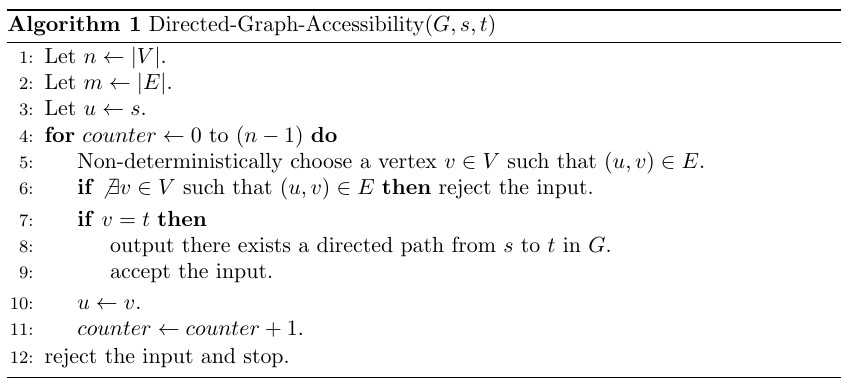
\includegraphics[scale=1.0]{Algo1-DGA.jpg}\end{center}
\end{figure}
The non-deterministic Turing machine that implements the above Directed-Graph-Accessibility$(G,s,t)$ algorithm needs atmost $O(\log n)$ space to store vertices $u,v\in V$, to store variables $n,m$ and to update the variable $counter$. In addition it looks up to the adjacency matrix of the directed graph given as input to find and non-deterministically choose vertex $v$ which is the head of the directed edge $(u,v)$ in each iteration. Clearly this also needs atmost $O(\log n)$ space.

Now, if there exists a directed path from $s$ to $t$ then any such path is of length less than or equal to $(n-1)$ and it is possible to non-deterministically guess the vertices along a directed path from $s$ to $t$. Thus whenever there exists a directed path there exists a computation path of the computation tree of this non-deterministic Turing machine that accepts. Conversely, if there is no path from $s$ to $t$ in $G$ then no computation path of this non-deterministic Turing machine ends in an accepting state. Therefore $\rm DSTCON\in\NL$.
\end{proof}

\begin{theorem}\label{DSTCONisNLcomplete}
{\rm DSTCON} is complete for $\NL$ under $\Lredn$ reductions.
\end{theorem}
\begin{proof}
The result follows from Lemma \ref{DSTCONisinNL} and Lemma \ref{DSTCONisNLhard}.
\end{proof}

\begin{definition}
We define $\LDAG =\{ G|G=(V,E)$ is a simple layered directed acyclic graph which does not have any self-loops on vertices or directed cycles or parallel edges between vertices. Also vertices in $G$ are arranged as a square matrix such that there are $n$ rows and every row has $n$ vertices. Any edge in this graph is from a vertex in the $i^{th}$ row to a vertex in the $(i+1)^{st}$ row, where $1\leq i\leq (n-1)$ and $n\geq 2\}$.
\end{definition}
\begin{figure}[h!]
\begin{center}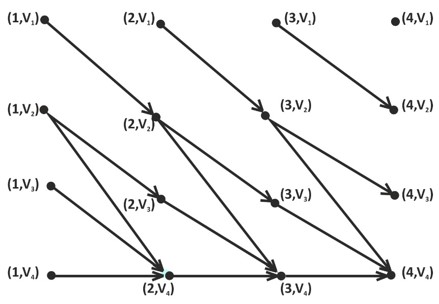
\includegraphics[scale=1.5]{SLDAGSTCON-instance.jpg}\end{center}
\caption{\it The above figure is a directed graph $G$ which is an instance of $\LDAG$. Assuming that vertices $s=(1,V_1)$ and $t=(4,V_4)$ we also infer that this instance $(G,s,t)$ is in $\LDAGSTCON$.}
\end{figure}
\begin{definition}\label{sharpL}
Let $\Sigma$ be the input alphabet. The complexity class $\sharpL$ is defined to be the class of functions $f:\Sigma^{*}\rightarrow\Z^{+}$ such that there exists a $\NL$ Turing machine $M$ for which we have $f(x)=\acc _M(x)$ where $\acc _M(x)$ denotes the number of accepting computation paths of $M$ on any input $x\in\Sigma^{*}$.
\end{definition}
\begin{definition}\label{sldagstcon}
Let $G=(V,E)\in \LDAG$ and $s,t\in V$ such that $s$ is a vertex in the first row and $t$ is a vertex in the last row of $G$. We define $\LDAGSTCON =\{ (G,s,t)|\exists$ a directed path from $s$ to $t$ in $G\}$.
\end{definition}

\begin{theorem}\label{sldagstconcomplete}
$\LDAGSTCON$ is complete for $\NL$ under logspace many-one reductions.
\end{theorem}
\begin{proof}
We know from Theorem \ref{DSTCONisNLcomplete} that the $st$-connectivity problem for directed graphs is complete for $\NL$ under logspace many-one reductions.
\begin{figure}[h!]
\begin{center}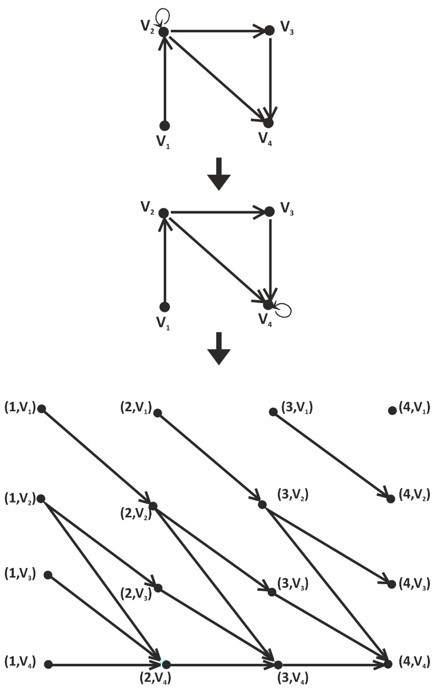
\includegraphics[scale=1.2]{SLDAGSTCON-reduction.jpg}\end{center}
\caption{\it The above figure explains the reduction from a directed graph $G_1$ with vertices $s_1=V_1$ to the vertex $t_1=V_4$ to a ``yes" instance $G$ of $\LDAGSTCON$ where $s=(1,V_1)$ and $t=(4,V_4)$.}
\end{figure}
Therefore the $st$-connectivity problem for directed graphs that do not have any self-loops on vertices or parallel edges between vertices is also complete for $\NL$ under logspace many-one reductions. In other words the $st$-connectivity problem for simple directed graphs is complete for $\NL$ under logspace many-one reductions. Let $G=(V,E)$ be a simple directed graph and $s,t\in V$. Also let $n=|V|$. Given $G$, we obtain the directed graph $G'=(V',E')$, where $V'=V$ and $E'=E\cup {(t,t)}$. We now reduce $G'$ to $G''=(V'',E'')\in \LDAG$. In $G''$, the vertex set $V''$ has $n^2$ vertices arranged as a $n\times n$ matrix obtained by creating $n$ copies of $V'$. As an example refer to the figure given below in which we obtain an instance of $\LDAG$ from the directed graph given as input. For the sake of convenience, we assume in this example that the vertices in each row of the instance of $\LDAG$ are arranged vertically.

Now let the vertex $s$ in the first row be denoted by $(1,s)$ and the vertex $t$ in the last row be denoted by $(n,t)$. A $(i,j)$ vertex in $G''$ is the $j^{th}$ vertex in the $i^{th}$ row of $G''$, where $1\leq i,j\leq n$. Here $E''=\{ ((i,j_1),(i+1,j_2))|(j_1,j_2)\in E'{\rm ,~where~}1\leq i\leq n-1{\rm ~and~} 1\leq j_1,j_2\leq n\}$. Now it is easy to note that there exists a directed path from $s$ to $t$ in $G$ if and only if there exists a directed path from $(1,s)$ to $(n,t)$ in $G''$. Since we can obtain $G''$ from $G$ using a logspace many-one reduction the result follows.
\end{proof}

\begin{corollary}\label{sldagcountsharplcomplete}
Let $(G,s,t)$ be an input instance of $\LDAGSTCON$. Then counting the number of directed paths from $s$ to $t$ in $G$ is complete for $\sharpL$ under logspace many-one reductions.
\end{corollary}

\begin{corollary}\label{parsicomplete}
Let $\Sigma$ be the input alphabet and $f\in \sharpL$ using a $\NL$ machine $M$ such that $f(x)=\acc_M(x)$ on any input $x\in \Sigma^*$. Then for an input string $x\in \Sigma^*$, $g(x)=(G,s,t)$, where $g$ is the canonical logspace many-one reduction used to show that $\LDAGSTCON$ is $\NL$-complete and $(G,s,t)$ is an input instance of $\LDAGSTCON$, and $f(x)$ is equal to the number of directed paths from $s$ to $t$ in $G$.
\end{corollary}
\section{Reducibilities based on oracles}\label{Chap01-Sec-Reduceoracle}
\begin{definition}
Let $\Sigma$ be the input alphabet and $L_1,L_2\in\Sigma^*$. We say that $L_1$ is logspace Turing reducible to $L_2$, denoted by $L_1\LTredn L_2$, if there exists a $O(\log n)$ space bounded Turing machine $M$ that has $L_2$ as an oracle such that given any input string $x\in\Sigma^*$, we have $M^{L_2}(x)$ accepts if and only if $x\in L_1$.
\end{definition}

\begin{definition}
Let $\Sigma $ be the input alphabet and let $\mathcal{C}$ be a complexity class. We define $\L^{\mathcal{C}}$ as the class of all languages $L\subseteq\Sigma^*$ that is accepted by a $O(\log n)$ space bounded deterministic Turing machine that has oracle access to a language $A\in\mathcal{C}$, where $n$ is the size of the input and $A\subseteq\Sigma^*$.
\end{definition}

It is easy to note that if $L_1$ is logspace Turing reducible to $L_2$ and $L_2$ is in a complexity class $\mathcal{C}$ where $\mathcal{C}$ contains the complexity class $\L$ of all languages that can be decided in deterministic logarithmic space then $L_1$ is in $\L^{\mathcal{C}}$.

\begin{definition}
Let $\Sigma$ be the input alphabet and let $\mathcal{C}$ be a complexity class. Then $L\subseteq \Sigma^*$ is logspace Turing hard for $\mathcal{C}$ if for any $L'\in\mathcal{C}$, we have $L'\LTredn L$.
\end{definition}

\begin{definition}
Let $\Sigma$ be the input alphabet and let $\mathcal{C}$ be a complexity class. Then $L\subseteq \Sigma^*$ is logspace Turing complete for $\mathcal{C}$ if $L\in\mathcal{C}$ and $L$ is logspace Turing hard for $\mathcal{C}$.
\end{definition}

\begin{definition}
Let $\Sigma $ be the input alphabet and let $\mathcal{C}$ be a complexity class. We define $\NL^{\mathcal{C}}$ to be the class of all languages $L\subseteq\Sigma^*$ that is accepted by a $O(\log n)$ space bounded non-deterministic Turing machine $M$ that has oracle access to a language $A\in\mathcal{C}$, where $n$ is the size of the input and $A\subseteq\Sigma^*$. Here we assume that $M$ makes queries to the oracle $A$ according to the Ruzzo-Simon-Tompa oracle access mechanism.
\end{definition}

\section{The Immerman-Szelepcs$\rm\acute{e}$nyi Theorem}\label{chap02-immermanszelepcsenyitheorem}
\subsection{The Immerman-Szelepcs$\acute{\bf e}$nyi Theorem in the logarithmic space setting}
\begin{theorem}\label{chap2-NLcomplement}
{$\boldNL =\boldcoNL$}
\end{theorem}
\begin{proof}
Let $G=(V,E)$ be an input instance of $\LDAG$ that is given as an adjacency matrix and let $s,t\in V$ such that $s$ is a vertex in the first row and $t$ is a vertex in the last row of $G$. We know from Theorem \ref{sldagstconcomplete} that deciding if $(G,s,t)\in\LDAGSTCON$ is complete for $\NL$ under logspace many-one reductions. Therefore to prove our result it suffices to prove that the problem of deciding if there does not exist any path from $s$ to $t$ in $G$ is also in $\NL$. In other words we show that $\overline{\LDAGSTCON}\in\NL$. Now let us consider the algorithm IS-Logspace($G,s,t$). 
\begin{figure}[htbp]
\begin{center}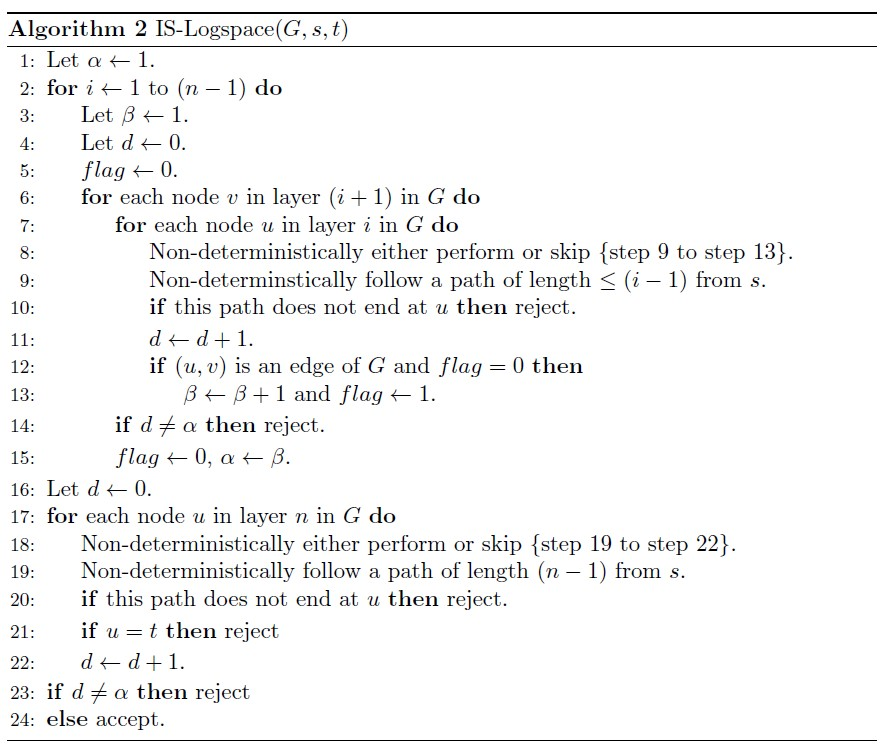
\includegraphics[scale=1.0]{Algo1-IS-Logspace.jpg}\end{center}
\end{figure}

We show that the above algorithm can be implemented by a $\NL$ Turing machine $M$. Then $M$ must have at least one accepting computation path whenever there does not exist any directed path from $s$ to $t$ in $G$.

Now assume that we know $\alpha$ which is the number of nodes in layer $n$ of $G$ that are reachable from from $s$ in $G$. We assume that $\alpha$ is provided as an input to $M$ and we show in steps 16 to 24 of the above algorithm IS-Logspace($G,s,t$), that it is possible to use $\alpha$ to prove that $\overline{\LDAGSTCON}\in\NL$ using a method which we call as {\bf \emph{non-deterministic counting}}. Later we prove that $M$ also computes $\alpha$ in steps 1 to 15 using the same non-deterministic counting method.

Given $G,s,t$ and $\alpha$, the Turing machine $M$ operates as follows. One by one $M$ goes through all the $n$ nodes in layer $n$ of $G$ and non-deterministically guesses whether each one is reachable from $s$. Whenever a node $u$ is guessed to be reachable, $M$ attempts to verify this guess by guessing a path of length $n$ or less from $s$ to $u$. If this computation branch fails to verify this guess, it rejects. The Turing machine $M$ counts the number of nodes that have been verified to be reachable. When a branch has gone through all of $G$'s nodes, it checks that the number of nodes that are verified to be reachable from $s$ equals $\alpha$, the number of nodes that are actually reachable from $s$, and rejects if not. Otherwise this computation branch accepts.

In other words, if $M$ non-deterministically selects exactly $\alpha$ nodes reachable from $s$, not including $t$, and proves that each is reachable from $s$ by guessing the path, $M$ knows that the remaining nodes including $t$ are not reachable and therefore it can accept.

Next we show in steps 1 to 15 described in the above algorithm IS-Logspace($G,s,t$), how to calculate $\alpha$: the number of nodes that are reachable from $s$ in layer $n$ in $G$. We describe a non-deterministic logspace procedure whereby at least one computation branch has at least the correct value of $\alpha$ in which it accepts and all the other branches reject.

Let $A_0=\{s\}$. For each $i$ from $1$ to $(n-1)$, we define $A_i$ to be the collection of all  nodes in layer $(i+1)$ that are reachable from $s$ by a directed path of length $i$. So $A_{n-1}$ is the set of all nodes in layer $n$ that are reachable from $s$ by a directed path of length $(n-1)$. Let $\beta=|A_{i-1}|$. Then in steps 6 to 15 of the IS-Logspace($G,s,t$) algorithm we show how to calculate $|A_i|$ from $|A_{i-1}|$. Repeated application of this procedure yields the desired value of $\alpha$.

We calaulate $|A_i|$ from $|A_{i-1}|$ using an idea similar to the one presented earlier in this proof. In the algorithm we go through all the nodes of $G$ in layer $(i+1)$ and determine whether each is a member of $A_i$ and also count the members to find $|A_i|$.

To determine whether a node $v$ is in $A_i$, we use an inner loop to go through all the nodes of $G$ in layer $i$ and guess whether each node is in $A_{i-1}$. Each positive guess is verified by a path of length $i$ from $s$. For each node $u$ verified to be in $A_{i-1}$, the algorithm tests whether $(u,v)$ is an edge of $G$. If it is an edge, $v$ is in $A_i$. Additionally the number of nodes verified to be in $A_{i-1}$ is counted. At the completion of the inner loop, if the total number of nodes verified to be in $A_{i-1}$ is not $\alpha$ then entire $A_{i-1}$ has not been found, so this computation branch rejects. If the count equals $\alpha$ and $v$ has not shown to be in $A_i$, we conclude that it is not in $A_i$. Then we go on to the next $v$ in layer $(i+1)$ in the outer loop. Since we use constant number of variables each of which takes values from $0$ to $n$ in the above algorithm IS-Logspace($G,s,t$), it is easy to note that the Turing machine $M$ that implements it is a $\NL$ Turing machine. As a result we have shown that $\overline{\LDAGSTCON}\in\NL$ which implies $\coNL\subseteq\NL$ from which the result follows.
\end{proof}

\begin{theorem}\label{nlclosureunderTuring}
$\boldL^{\boldNL}=\boldNL$
\end{theorem}
\begin{proof}
It is trivial to note that $\NL\subseteq\L^{\rm{\NL}}$. Now to prove our result we have to show that $\L^{\NL}\subseteq\NL$. Let $L'\in\L^{\NL}$. Then there exists a $\NL$ oracle Turing machine $M$ that has access to a language $A\in\NL$ as an oracle such that given any string $x\in\Sigma^*$, $M^A$ decides if $x\in L'$ correctly. Since $M$ is $O(\log n)$ space bounded, we infer that the number of queries that $M$ submits to the oracle $A$ is a polynomial in the size of the input. Let $M_A$ be the $\NL$ machine that decides if an input string is in $A$ or not. Due to Theorem \ref{chap2-NLcomplement} it follows that $\overline{A}$ is also in $\NL$. Let $M_{\overline{A}}$ be the $\NL$ machine that correctly decides if any input string is in $\overline{A}$. Now let $\Sigma$ be the input alphabet and let $x\in\Sigma^*$ be the input string. Let us consider the following algorithm implemented by a Turing machine $N$.

1. $N$ simulates $M$ on $x$ until a query $y$ is generated.

2. $N$ simulates $M_A$ on input $y$.

3. If $M_A$ accepts $y$ then $N$ continues to simulate $M$ on $x$ assuming the reply of the oracle is ``yes". Otherwise if $M_A$ rejects $y$ then $N$ simulates $M_{\overline{A}}$ on $y$. If $M_{\overline{A}}$ accepts $y$ then $N$ assumes the reply of the oracle is ``no" and continues to simulate $M$ on $x$. However if both $M_A$ and $M_{\overline{A}}$ reject $y$ then $N$ rejects the input string $x$.

We now show that $N$ correctly decides if $x\in L$. It is easy to note that if for any oracle query sring $y$, either $M_A$ or $M_{\overline{A}}$ can accept $y$ but not both. Also if $M_A$ accepts $y$ then $y\in A$. Similarly if $M_{\overline{A}}$ accepts $y$ then $y\in\overline{A}$. As a result when either of these two $\NL$ machines accept then this can be taken to be the output of the oracle and $N$ will proceed with its simulation of $M$. On the contrary if neither $M_A$ nor $M_{\overline{A}}$ accept since $\NL$ is closed under complement we know that there exists at least one accepting computation path in exactly one of these Turing machines and we did not simluate both the Turing machines along any such path. Therefore $N$ also rejects $x$ and stops the computation. Since $N$ simulates only $\NL$ Turing machines, it shows that $N$ is also a $\NL$ Turing machine. This shows that $\L^{\NL}\subseteq\NL$ from which we get that $\L^{\NL}=\NL$.
\end{proof}

Now the following result is easy to prove.
\begin{proposition}\label{nlunionintersection}
$\NL$ is closed under union and intersection.
\end{proposition}

\begin{theorem}\label{chap2-NLhierarchycollapses}
$\boldNL^{\boldNL}=\boldNL$
\end{theorem}
\begin{proof}
It is trivial to note that $\NL\subseteq\NL^{\rm{\NL}}$. Therefore we have to prove that $\NL^\NL\subseteq\NL$. Let $L\in\NL^\NL$. Then there exists a $\NL$ oracle Turing machine $M$ that has access to a language $A\in\NL$ as an oracle such that given any string $x\in\Sigma^*$, $M^A$ decides if $x\in L$ correctly. It follows from Section \ref{chap1-NOTM-model1} that this $\NL$ oracle Turing machine follows the Ruzzo-Simon-Tompa oracle access mechanism to submit queries to the oracle $A$. Also we infer from Section \ref{chap1-NOTM-model1} that the number of queries that are submitted to the oracle $A$ is a polynomial in the size of the input. Let $M_A$ be the $\NL$ machine that decides if an input string is in $A$ or not. Since we have shown in Theorem \ref{chap2-NLcomplement} that $\NL$ is closed under complement, it follows that $\overline{A}$ is also in $\NL$. Let $\overline{M_A}$ be the $\NL$ machine that correctly decides if any input string is in $\overline{A}$. Now let $\Sigma$ be the input alphabet and let $x\in\Sigma^*$ be the input string. Let us consider the following algorithm implemented by a Turing machine $N$: 

1. $N$ simulates $M$ on $x$ until a query $y$ is generated.

2. $N$ simulates $M_A$ on input $y$. If $M_A$ accepts $y$ then $N$ continues to simulate $M$ on $x$ assuming the reply of the oracle is ``yes". Otherwise if $M_A$ rejects $y$ then $N$ simulates $\overline{M_A}$ on $y$. If $\overline{M_A}$ accepts $y$ then $N$ assumes the reply of the oracle is ``no" and continues to simulate $M$ on $x$. However if both $M_A$ and $\overline{M_A}$ reject $y$ then $N$ rejects the input string $x$.

We now show that $N$ correctly decides if $x\in L$. It is easy to note that if for any oracle query sring $y$, either $M_A$ or $\overline{M_A}$ can accept $y$ but not both. Also if $M_A$ accepts $y$ then $y\in A$. Similarly if $\overline{M_A}$ accepts $y$ then $y\in\overline{A}$. As a result when either of these two $\NL$ machines accept then this can be taken to be the output of the oracle and $N$ will proceed with its simulation of $M$. On the contrary if neither $M_A$ nor $\overline{M_A}$ accept since $\NL$ is closed under complement we know that there exists at least one accepting computation path in exactly one of these Turing machines and we did not simluate both the Turing machines along any such path. Therefore $N$ also rejects $x$ and stops the computation. Since $N$ only simulates $\NL$ Turing machines it shows that $N$ is also a $\NL$ machine. This shows that $\NL^{\NL}=\NL$.
\end{proof}

\begin{theorem}\label{chap2-2SATisinNL}
Let {\rm 2SAT}=$\{\phi|\phi$ {~is~a~Boolean~formula~in~the~}2-CNF{~such~that~$\phi$ ~is~satisfiable\}}. Then ${\rm 2SAT}~{is~in~\NL}$ and $\overline{\rm 2SAT}~{is~in~\NL}$
\end{theorem}
\begin{proof}
We want to show that the language of all unsatisfiable Boolean formulas in the 2-CNF, denoted by $\overline {\rm 2SAT}$, is in $\NL$. Let $\phi=(\phi _1\wedge\phi _2\wedge\cdots\wedge\phi_m)$ be in 2-CNF. We assume without loss of generality that each $\phi _i$ is a conjunction of two literals, where $1\leq i\leq m$. Otherwise if there exists a clause $\phi _i$ that contains only one literal then we convert such a clause $\phi_i$ of $\phi$ into a conjunction of two new clauses where the first of the new clauses is a disjunction of the literal that occurs in $\phi _i$ along with a new variable $y$ which is not in the 2-CNF Boolean formula $\phi$ given as input and the second new clause is the disjunction of the literal that occurs in $\phi _i$ and $\neg y$. It is easy to observe that the resulting 2CNF Boolean formula is satisfiable if and only if $\phi$ is satisfiable. Note that we use only one new variable $y$ that is not in the 2-CNF Boolean formula $\phi$ given as input to convert all clauses that have only one literal into clauses that are the disjunction of two literals.

Now given a 2-CNF Boolean formula $\phi$ we define a directed graph $G=(V,E)$ as follows. For each variable $x$ that occurs in $\phi$ we define two vertices in $G$. More precisely, we define a vertex for the variable $x$ and a vertex for $\neg x$. Clearly if there are $n$ variables in $\phi$ then there are $2n$ vertices in $G$. If $\phi _i=(\neg x\vee y)$ is a clause then we include directed edges $(x,y)$ and $(\neg y,\neg x)$ in $E$ of $G$. In other words, if we have a clause of $\phi$ to be $(\neg x\vee y)$ which is $(x\Rightarrow y)$ then we include the directed edge $(x,y)$ in $E$. By commutativity, since $(\neg x\vee y)$ is also $(y\vee \neg x)$ which is $(\neg y\Rightarrow\neg x)$ we also include the edge $(\neg y,\neg x)$ in $E$ of $G$. Clearly if there are $m$ clauses in $\phi$ then there are $2m$ directed edges in $G$. Also it is easy to observe that there exists a directed path from a vertex $\alpha$ to a vertex $\beta$ in $G$ if and only if then there exists a directed path from $\neg \beta$ to $\neg \alpha$ in $G$. The 2-CNF Boolean formula $\phi$ is the conjunction of implications of the form $(\alpha\Rightarrow\beta )$, where $\alpha$ and $\beta$ are literals in the clauses of $\phi$. Given the conjunction of two clauses $(\alpha\Rightarrow\beta )\wedge (\beta\Rightarrow\gamma )$ we can simplify this conjunction and derive the clause $(\alpha\Rightarrow\gamma )$ from them. Using this we infer that the 2-CNF Boolean formula $\phi$ is unsatisfiable if and only if we can obtain a contradiction which is that there exists at least one variable $x$ such that we can simplify the conjunction of clauses in $\phi$ to obtain the clause $(x\Rightarrow \neg x)$ and also that $(\neg x\Rightarrow x)$. However this is equivalent to the existence of edges in $E$ of $G$ such that there is a directed path from $x$ to $\neg x$ and a directed path from $\neg x$ to $x$.

Now given a 2-CNF Boolean formula $\phi$ such that $n$ is the size of $\phi$, a $O(\log n)$-space bounded deterministic Turing machine can output the directed graph $G$ described above. We then use a $\NL$ oracle to query if there exists a directed path from a variable $x$ to $\neg x$ and also from $\neg x$ to $x$ in $G$ for all the variables $x$ that occur in $\phi$. If for some variable $x$ we get the oracle reply to be ``YES" for the queries submitted then we accept $\phi$ and output that $\phi$ is unsatisfiable. Otherwise we reject the input $\phi$ and output that $\phi$ is satisfiable. Now it follows from Theorem \ref{chap2-NLhierarchycollapses} that $\overline{\rm 2SAT}$ is in $\NL$.
\end{proof}

\begin{theorem}\label{chap2-2SATisNLhard}
{$\overline{\rm 2SAT}~{is~hard~for~\NL}~{under~\Lredn}~$${reductions}$}
\end{theorem}
\begin{proof}
We prove this statement by showing that ${\rm DSTCON}\Lredn\overline{\rm 2SAT}$. Let $G=(V,E)$ be a directed graph and let $(G,s,t)$ be the input instance of DSTCON. Let $n=|V|$. We construct a 2CNF Boolean formula $\phi$ from $(G,s,t)$ such that there exists a directed path from $s$ to $t$ in $G$ if and only if $\phi$ is not satisfiable. Let $x$ be the Boolean variable corresponding to the vertex $s$ in $G$ and $\overline{x}$ be the literal corresponding to the vertex $t$. For each of the remaining vertices $v_i$ in $G$, let there be a Boolean variable $x_i$. For each edge $(v_i,v_j)\in E$ let us include the clause $(v_i\Rightarrow v_j)$ in $\phi$. In other words, for each edge $(v_i,v_j)\in E$ we include the clause $(\overline{v_i}\vee v_j)$ in $\phi$. Apart from these clauses we also include the conjunction of the clause $(x)$ in $\phi$. Since the clause $(x)$ is not a disjunction of two distinct literals we introduce a new variable $y$ and include the conjunction of the following 2CNF Boolean subformula $(x\vee y)\wedge (x\vee \neg y)$ in $\phi$. Clearly a $O(\log n)$-space bounded deterministic Turing machine can output $\phi$ given $(G,s,t)$ as input.

Now consider the case when there exists a directed path from $s$ to $t$ in $G$. Let the vertices that form the directed path be the following in sequence: $s,v_i,v_j,\ldots ,v_k,t$, where $1\leq i,j,k\leq n$. We claim that $\phi$ is not satisfiable. To prove this claim consider the case when $x=F$. Then $\phi$ is not satisfiable since we have clauses $(x\vee y)\wedge (x\vee \neg y)$ in $\phi$. For the case when $x=T$ let us consider the 2CNF Boolean subformula of $\phi$ formed by the clauses due to the edges in a directed path from $s$ to$t$ in $G$: $(\overline{x}\vee v_i)\wedge (\overline{v_i}\vee v_j)\wedge\cdots\wedge (\overline{v_k}\vee \overline{x})$. It is easy to see that the Boolean subformula $(\overline{x}\vee v_i)\wedge (\overline{v_i}\vee v_j)\wedge\cdots\wedge (\overline{v_k}\vee \overline{x})$ is not satisfiable and so $\phi$ is also not satisfiable. Conversely, assume that there does not exist any directed path from $s$ to $t$ in $G$. Let $A$ be the subset of vertices in $V$ that are reachable from $s$ in $G$, $B$ be the subset of vertices in $V$ from which $t$ is reachable and $C=V\setminus (A\cup B)$. Since there is no directed path from $s$ to $t$ in $G$ it is easy to observe that the subsets of $V$ of vertices in $A,B$ and $C$ are pairwise disjoint and there are no edges from $A$ to $B\cup C$ and from $A\cup C$ to $B$ in $G$. Now let us assign the truth value $T$ to every variable in $A\cup C$ including the variable $x$ and the truth value $F$ to every variable in $B$ including the literal $\overline{x}$. It is easy to verify that this truth value assignment satisfies $\phi$. This shows that ${\rm DSTCON}\Lredn\overline{\rm 2SAT}$.
\end{proof}

\begin{theorem}
{${\rm 2SAT}~{is~complete~for~\NL}~{under~\Lredn}~$${reductions}$}
\end{theorem}
\begin{proof}
This result follows from Theorem \ref{chap2-2SATisinNL}, Theorem \ref{chap2-2SATisNLhard} and Theorem \ref{chap2-NLcomplement}.
\end{proof}

{\bf\underline{CONJECTURE}}: $\sharp$2SAT is complete for $\sharpL$ under $\Lredn$ reductions.

\subsection{Nondeterministic space bounded complexity classes above $\boldNL$}
\begin{definition}
Let $\Sigma$ be the input alphabet and $S(n)\in\Omega (\log n)$. We define the complexity class $\NSPACE (S(n))=\{ L\subseteq \Sigma^*|\exists$ a $O(S(n))$ space bounded non-deterministic Turing machine M such that $L=L(M)\}$.
\end{definition}

\begin{definition}
Let $\Sigma$ be the input alphabet and $S(n)\in\Omega (\log n)$. We define the complexity class $\coNSPACE (S(n))=\{ \overline{L}\subseteq \Sigma^*|L\in\NSPACE (S(n))\}$.
\end{definition}

\begin{theorem}
{\rm \bf(The Immerman-Szelepcs$\acute{\rm\bf e}$nyi Theorem)} $\NSPACE(S(n))=\coNSPACE (S(n))$, where $S(n)\in\Omega(\log n)$.
\end{theorem}
\begin{proof}
Let $\Sigma$ be the input alphabet and let $L\subseteq \Sigma^*$ such that $L\in\NSPACE (S(n))$. Let $M$ be the $\NSPACE(S(n))$ Turing machine that accepts $L$. As in the proof of Lemma \ref{DSTCONisNLhard} we observe that given an input $x\in\Sigma^*$, all the configurations of $M(x)$ is computable by a determinisitic Turing machine using space atmost $O(S(n))$ and therefore the directed configuration graph of $M(x)$ can also be output by a $O(S(n))$ space bounded deterministic Turing machine. As in Theorem \ref{sldagstconcomplete} we observe that the directed $st$-connectivity problem for the simple layered directed acyclic graph obtained from the directed configuration graph $G$ of a $\NSPACE (S(n))$ Turing machine $M(x)$ is a canonical complete problem for $\NSPACE (S(n))$. Now following the algorithm in the proof of Theorem \ref{chap2-NLcomplement} we are able to decide if there does not exist a directed path from a vertex $s$ in layer $1$ of the above graph $G$ to the vertex $t$ in layer $n$ of $G$ in $\NSPACE (S(n))$. This shows that $\coNSPACE (S(n))\subseteq \NSPACE (S(n))$ from which the theorem follows.
\end{proof}

\section{Logarithmic Space Bounded Counting classes}
In this section we assume without loss of generality that the input alphabet $\Sigma=\{ 0,1\}$. We informally say that a complexity class $\mathcal{C}$ is a logarithmic space bounded counting class if the criterion to decide if an input string $x\in\Sigma^*$ is in a language $L\in\mathcal{C}$ is based on the number of accepting computation paths and/or the number of rejecting computation paths of a $O(\log n)$ space bounded non-deterministic Turing machine $M$. We also call logarithmic space bounded counting classes that have access to oracles which are logarithmic space bounded counting classes as logarithmic space bounded counting classes. {\bf It follows from this informal definition that $\NL$ is the first and fundamental logarithmic space bounded counting class.}

We recall Definition \ref{sharpL}.
\begin{definition}
Let $\Sigma$ be the input alphabet. The complexity class $\sharpL$ is defined to be the class of functions $f:\Sigma^{*}\rightarrow\Z^{+}$ such that there exists a $\NL$ Turing machine $M$ for which we have $f(x)=\acc _M(x)$ where $\acc _M(x)$ denotes the number of accepting computation paths of $M$ on any input $x\in\Sigma^{*}$.
\end{definition}

\begin{definition}\label{GapL}
Let $\Sigma$ be the input alphabet. The complexity class $\GapL$ is defined to be the class of functions $f:\Sigma^{*}\rightarrow\Z$ such that there exists a $\NL$ machine $M$ for which we have $f(x)=\acc _M(x)-\rej _M(x)$ where $\acc _M(x)$ and $\rej _M(x)$ denote the number of accepting and the number of rejecting computation paths of $M$ on any input $x\in\Sigma^{*}$ respectively. We also denote $(\acc _M(x)-\rej _M(x))$ by $\gap _M(x)$.
\end{definition}

\begin{definition}\label{pldefinition}
A language $L$ belongs to the logarithmic space bounded counting class $\PL$ if there exists a $\GapL$ function $f$ such that $x\in L$ if and only if $f(x)>0$.
\end{definition}

\begin{definition}
A language $L$ belongs to the logarithmic space bounded counting class $\CeqL$ if there exists a $\GapL$ function $f$ such that $x\in L$ if and only if $f(x)=0$.
\end{definition}

We need the following result.
\begin{proposition}\emph{(Folklore)}\label{sharplfolklore}
\begin{enumerate}
\item Let $\Sigma$ be the input alphabet and $f:\Sigma^{*}\rightarrow\Z$ such that $f(x)\geq 0,~\forall x\in\Sigma^*$ and $f\in \FL$. Then $f\in\sharpL$.
\item $\sharpL$ is closed under addition.
\end{enumerate}
\end{proposition}
\begin{corollary}\label{nlproperty}
Let $\Sigma$ be the input alphabet and $L\subseteq\Sigma^*$ be a language in $\NL$. Then $\exists f\in\sharpL$ such that for any given input $x\in\Sigma^*$, we have $x\in L$ if and only if $f(x)\geq 2^{n^k}$, where $2^{n^k+1}$ is the number of computation paths of the $\NL$ Turing machine $M$ of $f$, and $k\geq 0$ is a constant.
\end{corollary}
\begin{proof}
Let $M'$ be the $\NL$ Turing machine that accepts $L$ such that on any input $x$ of length $n$ there are $2^{n^k}$ computation paths of $M'$ on $x$. For any given input $x\in\Sigma^*$, we know that $x\in L$ if and only if $acc_{M'}(x)>0$. Let $f(x)=acc_{M'}(x)+(2^{n^k}-1)$, where $n=|x|$. It follows from Proposition \ref{sharplfolklore} that $f\in\sharpL$. Also if $M$ is the $\NL$ Turing machine of $f$ then the number of computation paths of $M$ on any input $x$ of length $n$ is $2^{n^k+1}$. Clearly $x\in L$ if and only if $f(x)\geq 2^{n^k}$ which proves our result.
\end{proof}
\begin{corollary}\label{nlpropertyplusone}
Let $\Sigma$ be the input alphabet and $L\subseteq\Sigma^*$ be a language in $\NL$. Then $\exists g\in\sharpL$ such that for any given input $x\in\Sigma^*$, we have $x\in L$ if and only if $g(x)> 2^{n^k}$, where $2^{n^k+1}$ is the number of computation paths of the $\NL$ Turing machine $M$ of $g$, and $k\geq 0$ is a constant.
\end{corollary}
\begin{corollary}\label{nlpl}
$\NL\subseteq\PL$.
\end{corollary}
\begin{proof}
Follows from Definition \ref{pldefinition} and Corollary \ref{nlpropertyplusone}.
\end{proof}

\section{$\boldNL=\boldCeqL$}
%The results shown in this section are based on ideas from \cite[Lemma 3.7]{Tor1991}.
\begin{definition}
The symmetric difference of two sets $A$ and $B$ is the set of elements that belong to exactly one of $A$ and $B$. The symmetric difference of two sets $A$ and $B$ is denoted by $A\triangle B$. In other words, $A\triangle B=(\overline{A}\cap B)\cup (A\cap\overline{B})$.
\end{definition}
\begin{definition}
Let $\Sigma$ be the input alphabet. We define $(\NL\triangle\NL)=\{ L\subseteq\Sigma^*|\exists L_1,L_2\in\NL$ and $L=L_1\triangle L_2$, where $L_1,L_2\subseteq\Sigma^*\}$.
\end{definition}
We now deduce the following result from Corollary \ref{nlproperty} and Corollary \ref{nlpropertyplusone}.
\begin{theorem}\label{ceqlnldeltanl}
$\CeqL\subseteq(\NL\triangle\NL)$
\end{theorem}
\begin{proof}
Let $\Sigma$ be the input alphabet, $L\in\CeqL$ and let $M$ be a $\NL$ Turing machine such that on any input $x\in\Sigma^*$, we have $x\in L$ if and only if $gap_M(x)=0$. For any input $x\in\Sigma^*$ such that $n=|x|$, we assume without loss of generality that all the paths of the computation tree of $M$ on input $x$ have depth $n^k$, where $k>0$ is a constant and which clearly depends on the $O(\log n)$ space used by $M(x)$ along any of its computation paths. As a result the number of computation paths of $M(x)$ is $2^{n^k}$, and $x\in L$ if and only if $acc_M(x)=2^{n^k-1}$.

Consider the following. Let $L_1=\{x\in\Sigma^*|acc_M(x)\geq 2^{n^k-1}\}$ and let $L_2=\{x\in\Sigma^*|acc_M(x)>2^{n^k-1}\}$. It follows from Corollary \ref{nlproperty} and Corollary \ref{nlpropertyplusone} that $L_1,L_2\in\NL$. Also $L_2\subseteq L_1$ and we also deduce that $L=L_1\triangle L_2$. Thus $L\in\NL\triangle\NL$ which implies $\CeqL\subseteq(\NL\triangle\NL)$.
\end{proof}

\begin{theorem}\label{nldeltanllnl}
$(\NL\triangle\NL)\subseteq\L^{\NL}$.
\end{theorem}
\begin{proof}
Given two sets $A$ and $B$ it is easy to note that $(A\triangle B)=(\overline {A}\cap B)\cup (A\cap \overline{B})$. Now let $A,B\in\NL$. Due to Theorem \ref{chap2-NLcomplement} and Proposition \ref{nlunionintersection}, it follows that $(A\triangle B)\in\NL$. Clearly to determine if an input string $x\in\Sigma^*$ is in $(A\triangle B)$ a logarithmic space bounded deterministic Turing machine that has access to a $\NL$ oracle shall make one query and output if $x$ is in $(A\triangle B)$ or not. This shows that $(\NL\triangle\NL)\subseteq\L^{\NL}$.
\end{proof}

We therefore obtain the following result from Theorem \ref{ceqlnldeltanl}, Theorem \ref{nldeltanllnl} and Theorem \ref{nlclosureunderTuring}.
\begin{corollary}\label{ceqlnl}
$\CeqL\subseteq\NL$.
\end{corollary}

\begin{lemma}\label{nlcoceql}
$\NL\subseteq\coCeqL$.
\end{lemma}
\begin{proof}
Let $L\subseteq \Sigma^*$ such that $L\in\NL$ and let $M$ be the $\NL$-Turing machine which accepts $L$. Let $f\in\sharpL$ such that on any input $x\in\Sigma^*$ we have $f(x)=acc_M(x)~\forall x\in\Sigma^*$. For any input $x\in\Sigma^*$ such that $n=|x|$, we assume without loss of generality that all the paths of the computation tree of $M$ on input $x$ have depth $n^k$, where $k>0$ is a constant and which clearly depends on the $O(\log n)$ space used by $M(x)$ along any of its computation paths. Let us consider the following algorithm which can be implemented by a $\NL$-Turing machine, say $M'$, on a given input $x\in\Sigma^*$, where $n=|x|$:
\begin{quote}
Non-deterministically choose to either\newline \{simulate $M$ on input $x$\} or \newline \{form a computation tree having depth $n^k$ and accept the input $x$ on all of these computation paths\}.
\end{quote}
On any given input $x\in\Sigma^*$, if $x\in L$ then $f(x)\geq 1$. As a result $gap_{M'}(x)=acc_{M'}(x)-rej_{M'}(x)>0$. However if $x\not\in L$ then all the computation paths of $M$ on input $x$ end in the rejecting configuration and therefore $acc_{M'}(x)=rej_{M'}(x)$ which clearly implies $gap_{M'}(x)=0$. This shows that $L\in\coCeqL$ from which we get $\NL\subseteq\coCeqL$.
\end{proof}
\begin{theorem}\label{nlceql}
$\NL\subseteq\CeqL$.
\end{theorem}
\begin{proof}
From Lemma \ref{nlcoceql} we infer that $\coNL\subseteq \CeqL$. Also as a consequence of Theorem \ref{chap2-NLcomplement} we obtain that $\NL\subseteq\CeqL$.
\end{proof}
\begin{corollary}\label{nlequalsceql}
$\NL =\CeqL$.
\end{corollary}

\section{The Isolating Lemma}
Let $A = \{a_1,a_2,\ldots ,a_m\}$ be a set of elements and let $\F$ be a collection of non-empty subsets of $A$. Let $W$ be a finite number of consecutive integers, which are called as integer weights, and assume that we shall assign integer weights to elements of $A$ using a function $f:A\rightarrow W$. Define the weight of a subset $S$ of $A$, denoted by $f(S)$, to be the sum of the weights of the elements in the subset $S$.

We say that a weight function $f$\emph{ is good for }$\F$ if there is exactly one minimum-weight set in $\F$ with respect to $f$ and we say that $f$\emph{ is bad for }$\F$ otherwise.
\begin{theorem}{\textrm{\bf (The Isolating Lemma)}}\label{Isolating}
Let $A$ be a finite set of cardinality $m$ and let $\F$ be a family of non-empty subsets of $A$. Let $r>2m$ and let $f$ be a function $f:A\rightarrow\{1,\ldots ,r\}$ that assigns a value independently and uniformly at random to each element in $a_i\in A$ from the set $\{ 1,\ldots ,r\}$, where $1\leq i\leq m$. Then,
\[
Pr[f~is~good~for~\F ]\geq\frac{1}{2}.
\]
\end{theorem}
\begin{proof}
Let $MinWeight_f(\F )=\min \{f(S)|S\in\F\}$ and let $MinWeightSet_f(\F )=\{S\in\F |f(S)=MinWeight_f(\F )\}$. Recall from the definition of good and bad functions stated above that any weight function $f$ is bad for $\F$ if and only if $|MinWeightSet_f(\F )|\geq 2$.

For $x\in A$, we say that the minimum-weight sets of $\F$ with respect to $f$ are unambiguous about the inclusion of $x$ if there exists $S,S'\in MinWeightSet_f(\F )$ such that $x\in (S\setminus S')\cup (S'\setminus S)$. It is easy to note that $f$ is bad for $\F$ if and only if there exists some $x\in A$ such that the minimum-weight sets of $\F$ with respect to $f$ are ambiguous about the inclusion of $x$.

Now assume that the function $f$ is bad for $\F$. In other words, the minimum weight sets of $\F$ with respect to $f$ are ambiguous about the inclusion of $x$, for some $x\in A$. Let $f':A\rightarrow \{ 1,\ldots, r\}$ be another function such that for any $S\subseteq A$, if $x\not\in S$ then $f'(S)=f(S)$. However if $x\in S$ then $f'(S)\neq f(S)$ otherwise. 

{\emph{Claim.}} Minimum-weight sets of $\F$ with respect to $f'$ are unambiguous about the inclusion of $x$.

{\emph{Proof of Claim.}}
To prove this, let $\delta (x)=f'(x)-f(x)$. Suppose that $\delta (x)>0$. For any $S\subseteq A$, if $x\in S$ then $f'(S)=f(S)+\delta (x)$ and $f'(S)=f(S)$ otherwise. This implies that $MinWeight_f(\F )=MinWeight_{f'}(\F )$ and $MinWeightSet_{f'}(\F )=\{ S\in MinWeightSet_f(\F )|x\not\in S\}$. Next suppose that $\delta (x)<0$. Then, for all $S\in \F$, we have $f'(S)=f(S)-|\delta (x)|$ if $x\in S$ and $f'(S)=f(S)$ otherwise. This implies that $MinWeight_f(\F )=MinWeight_{f'}(\F )-|\delta (x)|$ and $MinWeightSet_{f'}(\F )=\{ S\in MinWeightSet_f(\F )|x\in S\}$. Therefore, if $\delta (x)>0$ then all the minimum-weight sets of $\F$ with respect to $f'$ contain $x$ and if $\delta (x)<0$ then there does not exist any minimum-weight set of $\F$ with respect to $f'$ that contains $x$. This proves our claim.

Now if there exists some $x\in A$ such that the minimum-weight sets of $\F$ with respect to $f$ are ambiguous about the inclusion of $x$, then certainly there exists an element $y\in A$ such that $y\neq x$ and the minimum-weight sets of $\F$ with respect to $f$ are ambiguous about the inclusion of $y$. If the number of such elements in $A$ is exactly $2$, then the number of functions $f'$ that we can obtain from $f$ as in the claim stated above such that these two minimum-weight sets of $\F$ with respect to $f'$ are unambiguous about the inclusion of $x,y$ is atmost $r^{m-2}$. Since there can be ${{m}\choose {2}}$ such pairs $x,y$, the number of such functions $f:A\rightarrow \{ 1,\ldots ,r\}$ is atmost ${{{m}\choose {2}}r^{m-2}}$. Note that not all of these functions have to be bad for $\F$. Extending this observation, if there were $k$ many such elements in $A$ such that the minimum-weight sets of $\F$ with respect to $f$ are ambiguous about the inclusion of any of these elements, then the number of functions that we can obtain from $f$ as done in the claim stated above is atmost ${{{m}\choose {k}}r^{m-k}}$. However this quantity is $\leq {mr^{m-1}}$. As a result, the proportion of functions $f$ such that $f$ is bad for $\F$ is $\leq\frac{mr^{m-1}}{r^m}\leq \frac{1}{2}$. Therefore the proportion of functions $f$ that are good for $\F$ is $\geq\frac{1}{2}$ and this proves our theorem.
\end{proof}

We recall the definition of $\DSTCON$ from Definition \ref{dstcon-defn}.
\begin{corollary}
Let $G=(V,E)$ be a directed graph which does not have any self-loops such that $s,t\in V$ and let $(G,s,t)$ be a ``yes" input instance of $\DSTCON$. Let us consider the function $f:E\rightarrow \{1,\ldots ,4|E|\}$ that assigns a value independently and uniformly at random to every edge in $E$ of $G$. Then,
\[
Pr[there~exists~a~directed~path~ from~s~to~t~in~G~that~has~unique~minimum~weight]\geq\frac{3}{4},
\]
where the weight of a directed path is the sum of the weights of the edges in the directed path.
\end{corollary}
\begin{proof}
We obtain this result by following the proof of Theorem \ref{Isolating}.
\end{proof}

\section{Uniqueness of directed paths in weighted directed graphs}
\begin{theorem}\label{family-Isolating}
Let $A$ be a finite set of cardinality $m$ and let $\F _1,\F _2,\ldots ,\F _n$ be families of non-empty subsets of $A$, where $n\leq m^k$ for some $k\geq 0$. Also let $r>\max (4m,4n)$. Then there exists a function $f:A\rightarrow\{1,\ldots ,r\}$ such that $f$ is good for every $\F _i$, where $1\leq i\leq n$.
\end{theorem}
\begin{proof}
We show this result using the following simple counting method, known as the Adleman's technique. Form a $0,1$ matrix $M$ of dimension $n\times r^n$ with $n$ rows and $r^n$ columns, where the $i^{th}$ row of $M$ corresponds to the family $\F _i$ and the $j^{th}$ column corresponds to the function $f_j$ in the lexicographically increasing order, for $1\leq i\leq n$ and $1\leq j\leq r^n$. (Here we assume that every function $f$ is considered as a vector, and given two functions $f$ and $g$ we say that $f$ is lexicographically lesser than $g$, denoted by $f\prec g$, if $f$ is lesser than $g$ when compared component-wise as vectors). We put $M_{ij}=1$ if the function $f_j$ is good for the family $\F _i$ and $M_{ij}=0$ otherwise. By the choice of $r$ and from the proof of Theorem \ref{Isolating}, it follows that
\[
{\rm Pr}\left[f~is~good~for~\F _i\right]\geq\frac{3}{4},
\]
where $f$ is a function chosen independently and uniformly at random, and $1\leq i\leq n$. Now using induction on $m$, it is easy to see that there exists a column in $M$ that contains only $1$. The function corresponding to this column satisfies the condition stated in this theorem.
\end{proof}

\begin{corollary}\label{min-unique-family-isolating}
Let $G=(V,E)$ be a directed graph which does not have any self-loops and let $m=|E|$. Let $n$ denote the number of ordered pairs of vertices $(s,t)$ such that there exists a directed path from $s$ to $t$ in $G$. Also let $r>\max (4m,4n)$. Then, we have a function $f:E\rightarrow\{1,\ldots ,r\}$ that assigns weights to the edges of $G$, such that there exists a directed path of unique minimum weight between every pair of vertices $(s,t)$ for which there exists a directed path from $s$ to $t$ in $G$, where the weight of a directed path is the sum of the weights of the edges in the directed path.
\end{corollary}
\begin{proof}
Given a directed graph $G=(V,E)$, the number of pairs of vertices between which there exists a directed path, denoted by $n$, is $\leq 2{{v}\choose {2}}$, where $v=|V|$. If $s,t\in V$ is such that there exists a directed path from $s$ to $t$ in $G$, then the set of edges corresponding to every directed path from $s$ to $t$ is a subset of $E$. Considering all directed paths from $s$ to $t$ we get the family of non-empty subsets of $E$, which we denote by $\F$. As a result there are $n$ families $\F_1,\ldots ,\F _n$. Also let $m=|E|$. Now apply Theorem \ref{family-Isolating} to obtain the function $f$ and this completes the proof.
\end{proof}

\section{Min-unique graphs and Unambiguous Logarithmic space: $\boldUL$}
\begin{definition}\label{minunique}
A min-unique graph is a directed graph with positive weights associated with each edge where for every pair of vertices $u,v$, if there is a path from $u$ to $v$, then there is a unique minimum weight path from $u$ to $v$. Here, the weight of a path is the sum of the weights on its edges.
\end{definition}
We now define the complexity class unambiguous logarithmic space, $\UL$.
\begin{definition}\label{UL}
Let $\Sigma$ be the input alphabet. We say that $L\subseteq\Sigma ^{*}$ is a language in the complexity class $\UL$ if there exists a function $f\in \sharpL$ such that for any input $x\in\Sigma ^{*}$ we have $f(x)=1$ if $x\in L$ and $f(x)=0$ if $x\not\in L$.
\end{definition}
We now define $\coUL$, based on the definition of $\mbox{co-}\mathcal{C}$ from Definition \ref{compdefinition} where $\mathcal{C}$ is a complexity class.
\begin{definition}\label{coUL}
Let $\Sigma$ be the input alphabet. For a language $L\in\Sigma^*$, the complement of $L$ is $\overline{L}=\Sigma^*-L$. We define the complexity class $\coUL=\{ \overline{L}\subseteq \Sigma ^*|L\in\UL\}$.
\end{definition}
\begin{definition}
Let $\Sigma$ be the input alphabet. We say that $L\in\UL\cap\coUL$ if $L\in\UL$ and $L\in\coUL$.
\end{definition}
\begin{theorem}\label{min-unique-st-connectivity-UL}
Let $\mathcal{G}$ be a class of graphs and let $H=(V,E)\in\mathcal{G}$. If there is a polynomially bounded logarithmic space computable function $f$ that on input $H$ outputs a weighted graph $f(H)$ so that
\begin{enumerate}
\item $f(H)$ is min-unique, and
\item $H$ has an $st$-path if and only if $f(H)$ has an $st$-path
\end{enumerate}
then the $st$-connectivity problem for $\mathcal{G}$ is in $\UL\cap\coUL$.
\end{theorem}
\begin{proof}
It suffices to give a $\UL\cap\coUL$ algorithm for the reduced graph. For $H\in\mathcal{G}$, let $G=f(H)$ be a directed graph with a min-unique weight function $w$ on its edges. We first construct an unweighted graph $G'$ from $G$ by replacing every edge $e$ in $G$ with a path of length $w(e)$. It is easy to see that $st$-connectivity is preserved. That is, there is an $st$-path in $G$ if and only if there is one in $G'$. Since $G$ is min-unique, it is straightforward to argue that the shortest path between any two vertices in $G'$ is unique.

Let $c_k$ and $\Sigma _k$ denote the number of vertices which are at a distance at most $k$ from $s$ and the sum of the lengths of the shortest path to each of them, respectively. Let $d(v)$ denote the length of the shortest path from $S$ to $v$.
\begin{figure}[htbp]
\begin{center}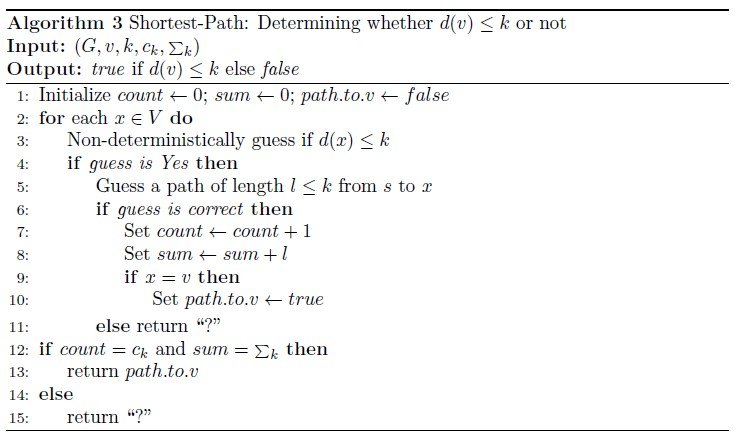
\includegraphics[scale=0.8]{Algo3-shortest_path.jpg}\end{center}
\end{figure}
If no such path exists, then $d(v)=|V|+1$. We have,
\[
{\ssum}_k=\sum_{\begin{array}{c}{\scriptstyle\{{v\in V}}|{\scriptstyle{d(v)\leq k}\}}\end{array}}d(v).
\]
We first give an unambiguous routine (Algorithm 3) to evaluate the predicate ``$d(v)\leq k$" when given the values of $c_k$ and $\ssum _k$. The algorithm will output the correct value of the predicate (\emph{true/false}) on a unique path and outputs ``?" on the rest of the paths.

We will argue that Algorithm 3 is unambiguous.
\begin{enumerate}
\item If Algorithm 3 incorrectly guesses that $d(x)>k$ for some vertex $x$ then $count<c_k$ and so it returns ``?" in line 18. Thus, consider the computation paths that correctly guess the set $\{ x|d(x)\leq k\}$.
\item If at any point the algorithm incorrectly guesses the length $l$ of the shortest path to $x$, then one of the following two cases occur.
\begin{enumerate}
\item If $d(x)>l$ then no path from $s$ to $x$ would be found and the algorithm returns ``?" in line 11.
\item If $d(x)<l$ then the variable \emph{sum} would be incremented by a value greater than $d(x)$ and thus \emph{sum} would be greater than $\ssum _k$ causing the algorithm to return ``?" in line 18.
\end{enumerate}
\end{enumerate}
Thus there will remain only one computation path where all the guesses are correct and the algorithm will output the correct value of the predicate on this unique path. Finally, we note that Algorithm 3 is easily seen to be computable in logarithmic space.
\begin{figure}[htbp]
\begin{center}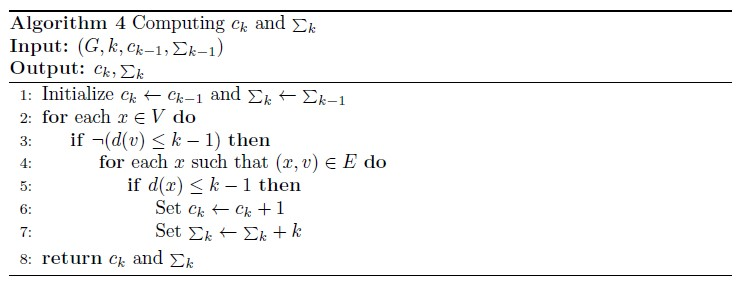
\includegraphics[scale=0.8]{Algo4-cksigmak.jpg}\end{center}
\end{figure}
\begin{figure}[htbp]
\begin{center}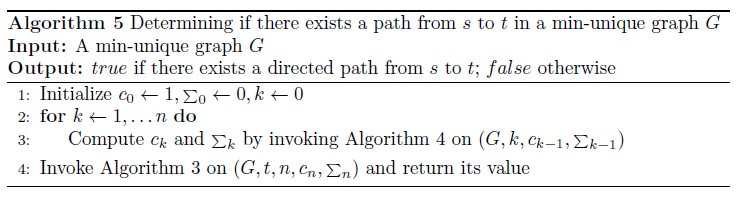
\includegraphics[scale=0.8]{Algo5-minuniquestconn}\end{center}
\end{figure}

Next, we describe an unambiguous procedure (Algorithm 4) that computes $c_k$ and $\ssum _k$ given $c_{k-1}$ and $\ssum _{k-1}$. Algorithm 4 uses Algorithm 3 as a subroutine. Other than calls to Algorithm 3, this routine is deterministic, and so it follows that Algorithm 4 is also unambiguous.

We will argue that Algorithm 4 computes $c_k$ and $\ssum _k$. The subgraph consisting only of $s$ $(d(x)\leq 0)$ is trivially min-unique and $c_0=1$ and $\ssum _0=0$. Inductively, it is easy to see that
\[
\begin{array}{c}
c_k=c_{k-1}+|\{ v|d(v)=k\}|,\\
\ssum _k=\ssum _{k-1}+k|\{v|d(v)=k\}|.
\end{array}
\]
In addition, $d(v)=k$ if and only if there exists $(x,v)\in E$ such that $d(x)\leq k-1$ and $\neg (d(v)\leq k-1)$. Both of these predicates can be computed using Algorithm 3. Combining these facts, we see that Algorithm 4 computes $c_k$ and $\ssum _k$ given $c_{k-1}$ and $\ssum _{k-1}$.

As a final step, we give the main routine that invokes Algorithm 4 to check for $st$-connectivity in a min-unique graph. Since there is an $st$-path if and only if $d(t)\leq n$, it suffices to compute $c_n$ and $\ssum _n$ and invoke Algorithm 3 on $(G,t,n,c_n,\ssum _n)$. This procedure is presented as Algorithm 5. To ensure that the algorithm runs in logarithmic space, we do not store all intermediate values for $c_k,\ssum _k$. Instead, we only keep the most recently computed values and re-use space. As with Algorithm 4, this procedure is deterministic and so the entire routine is unambiguous. Thus reachability in min-unique graphs can in fact be decided in $\UL\cap\coUL$.
\end{proof}

\section{$\boldNL {\rm\bf /poly} =(\boldUL\cap\boldcoUL ){\rm\bf /poly}$}
\begin{definition}\label{nonuniformC}
Let $\ssum =\{ 0,1\}$ be the input alphabet and let $\mathcal{C}$ be a complexity class. We define $\mathcal{C}/poly$ as the complexity class of all languages $L\subseteq\ssum^*$for which there exists a sequence of ``advice strings" $\{\alpha (n)|n\in \N\}$ and a language $L'\in\mathcal{C}$ such that $x\in L$ if and only if $(x,\alpha (x))\in L'$, where $x\in \ssum^*$.
\end{definition}
\begin{theorem}
$(\UL\cap\coUL){\rm /poly}\subseteq \NLpoly$.
\end{theorem}
\begin{proof}
It is easy to see from Definition \ref{UL} and Definition \ref{NLdefn} that $\UL\subseteq\NL$. Also we know from the Immerman-Szelepsc${\rm \acute{e}}$nyi Theorem (shown in Theorem \ref{chap2-NLcomplement}) that $\NL=\coNL$ and so $(\UL\cap\coUL)\subseteq\NL$. Using Definition \ref{nonuniformC}, it is now trivial to show that $(\UL\cap\coUL){\rm /poly}\subseteq \NLpoly$.
\end{proof}
\begin{theorem}
$\NLpoly\subseteq (\UL\cap\coUL){\rm /poly}$.
\end{theorem}
\begin{proof}
Using Definition \ref{nonuniformC}, we infer that it is sufficient to show that $\NL\subseteq (\UL\cap\coUL){\rm /poly}$. We know from Theorem \ref{DSTCONisNLcomplete} that, $\DSTCON$ is complete for $\NL$ under $\Lredn$. Therefore to prove our result, it is sufficient to show that $\DSTCON\in(\UL\cap\coUL){\rm /poly}$.

Let us now consider an input instance $(G,s,t)$ of $\DSTCON$. We assume without loss of generality that $G$ does not have any self-loops. It follows from Corollary \ref{min-unique-family-isolating} that, we have a function $f:E\rightarrow\{1,\ldots ,r\}$ that assigns weights to the edges of $G$, such that there exists a directed path of unique minimum weight between every pair of vertices $(s,t)$ for which there exists a directed path from $s$ to $t$ in $G$, where the weight of a directed path is the sum of the weights of the edges in the directed path.

Assume we are given an input instance $(G,s,t)$ of $\DSTCON$. Let the function stated in Corollary \ref{min-unique-family-isolating} be given as an advice string which is a vector of weights $\vec{\rm\bf w}=(w_1,w_2,\ldots ,w_m)$, where $m=|E|$. Clearly $\vec{\rm\bf w}$ is of length which is polynomial in the size of $(G,s,t)$. We observe that upon assigning weights to the edges of $G$ according to $\vec{\rm\bf w}$, the input directed graph $G$ is min-unique. Now using this advice string and Theorem \ref{min-unique-st-connectivity-UL}, it follows that we can decide if there exists a directed path from $s$ to $t$ in $G$ in $(\UL\cap\coUL )$. As a result it follows that 
$\DSTCON\in(\UL\cap\coUL){\rm /poly}$ which proves our result.
\end{proof}
\begin{theorem}
$\NLpoly=(\UL\cap\coUL){\rm /poly}$.
\end{theorem}

\chapter{Modulo-based and Probabilistic Logarithmic Space Bounded Counting Classes}
\section{Salient properties of $\boldGapL$}
\begin{lemma}\label{computationpathsupperbound}
Let $\Sigma$ be the input alphabet. If $f(x)$ is a $\sharpL$ or $\GapL$ function then there exists a polynomial $p(n)$ such that the absolute value of $f(x)$ is bounded above by $2^{p(n)}$ for every $x\in\Sigma^*$, where $n=|x|$.
\end{lemma}
\begin{proof}
Either $f(x)=acc _M(x)$ or $\gap _M(x)$ for some $\NL$ Turing machine $M$. Let $s(n)\in O(\log n)$ be an upper bound the amount of space that $M$ uses on input strings of length $n$. It is easy to note that the running time of $M(x)$ is at most $p(|x|)=2^{s(|x|)}$, which is a polynomial in $|x|$. As a result the number of distinct computation paths of $M$ on any input $x$ is upper bounded by $2^{p(|x|)}$ from which it follows that the number of  accepting and rejecting computation paths of $M$ on any input $x$ is at most $2^{p(|x|)}$ and this proves our claim.
\end{proof}

\begin{lemma}\label{gaplcomplement}
If $f\in\GapL$ then $-f\in\GapL$.
\end{lemma}

\begin{lemma}\label{chap06-gaplsharpl}
Let $\Sigma$ be the input alphabet. For every $\NL$ Turing machine $M$, there is a $\NL$ machine $N$ such that $\gap_N(x)=\acc_M(x)$ for every input $x\in\Sigma^*$.
\end{lemma}
\begin{proof}
Given an input $x$, the Turing machine $N$ guesses a path $p$ of $M(x)$. If $p$ is accepting, $N$ accepts. Otherwise, $N$ branches once, accepting on one branch and rejecting on the other. We have, for all $x$, $\gap_N(x)=\acc_N(x)-\acc_{\overline{N}}(x)=\acc_N(x)-\acc_{\overline{M}}(x)=(\acc_M(x)+\acc_{\overline{M}}(x))-\acc_{\overline{M}}(x)=\acc_M(x).$
\end{proof}
\begin{corollary}\label{corollary-gaplsharpl}
$\sharpL\subset\GapL$.
\end{corollary}
\begin{proof}
Follows from Lemma \ref{chap06-gaplsharpl} and the fact that $\GapL$ contains functions that take negative values on many inputs.
\end{proof}

Note that a $\sharpL$ function can take only nonnegative values and so this class cannot capture all the functions in $\FL$ that evaluate to integer values on any given input. However, it does capture those functions in $\FL$ that only take nonnegative integer values on all inputs. The class $\GapL$ encompasses any function in $\FL$ that takes integer values on any input without any restriction. For the rest of this chapter, we assume without loss of generality that any function $f\in \FL$ that we consider always takes integer values on any input.
\begin{theorem}
If an $\FL$ function $f$ always takes on nonnegative values then $f$ is in $\sharpL$. Every $\FL$ function $f$ is in $\GapL$.
\end{theorem}
\begin{proof}
Let $f$ be a $\FL$ function that always takes non-negative values. Define a $\NL$ Turing machine $M$, that on input $x$ guesses $f(x)$ computation paths and accepts on each of these paths.. Clearly $\acc_M(x)=f(x)$ when $f(x)\geq 0$, for all $x\in\Sigma^*$, where $\Sigma$ is the input alphabet.

Now let $f\in\FL$. Define a $\NL$ Turing machine $N$ which on input $x$ computes $f(x)$. For any $f(x)$ whether it is positive or negative, it follows from Corollary \ref{corollary-gaplsharpl} that there exists a NL Turing machine $N'$ such that $\gap_{N'}(x)=|f(x)|$. Therefore after computing $f(x)$, if $f(x)>0$ then $N$ simulates $N'$ on input $x$. However, if $f(x)<0$, then $N$ simulates $N'$ on input $x$ and rejects along the computation paths in which $N'$ accepts and accepts along the computation paths in which $N'$ rejects. This shows that $\gap_N(x)=f(x)$.
\end{proof}

\begin{lemma}
For all functions $f$, the following are equivalent:
\begin{enumerate}
\item $f\in\GapL$.
\item $f$ is the difference of two $\sharpL$ functions.
\item $f$ is the difference of a $\sharpL$ and $\FL$ function.
\item $f$ is the difference of a $\FL$ function and a $\GapL$ function.
\end{enumerate}
\end{lemma}
\begin{proof}
$(1\Rightarrow 2)$ For any $M$ we have $\gap_M(x)=\acc_M(x)-\acc_{\overline{M}}(x)$ by definition, so $\GapL$ is the difference of two $\sharpL$ functions.

$(2\Rightarrow 3)$ Let $f$ and $g$ be $\sharpL$ functions. We can assume that $f=\acc_M$ and $g=\acc_N$, where $M$ and $N$ are $\NL$ Turing machines, and $N$ has $2^{q(n)}$ computation paths for some polynomial $q$ (just pad $N$ with extra rejecting computation paths so that all computation paths have length $q(n)$). Let $M'$ be the $\NL$ Turing machine that first branches once, then simulates $M$ on one branch and $\overline{N}$ on the other. We have, for any $x$, $f(x)-g(x)=\acc_M(x)-\acc_N(x)=\acc_M(x)+\acc_{\overline{N}}(x)-2^{q(|x|)}=\acc_{M'}(x)-2^{q(|x|)}$. Therefore $f-g$ is the difference of a $\sharpL$ and a $\FL$ function.

$(3\Rightarrow 1)$ Let $f$ be a $\sharpL$ function and let $g\in\FL$. Let $M$ be the $\NL$ Turing machine such that $f=\gap_M(x)$. Let $N$ be such that, for all $x\in\Sigma^*$, $N(x)$ resembles $M(x)$ padded with $g(x)$ rejecting computation paths. We then have $\gap_N(x)=f(x)-g(x)$.

$(3\Leftrightarrow 4)$ This follows since we now have $(1\Leftrightarrow 3)$, and the $\GapL$ functions are closed under negation.
\end{proof}
\begin{corollary}\label{gaplequivsharpl}
$\GapL\subseteq\FL^{\sharpL{\mbox{\rm [1]}}}$.
\end{corollary}
\begin{proof}
Follows from the third characterization of $\GapL$ in the above lemma.
\end{proof}
The composition of two $\FL$ functions remains a $\FL$ function. However it seems unlikely that the composition of two $\sharpL$ functions is a $\sharpL$ or even a $\GapL$ function. We can however, combine $\sharpL$ and $\GapL$ functions with $\FL$ functions.
\begin{lemma}
Let $f$ be a $\FL$ function and $g$ a $\sharpL$ or $\GapL$ function. Then $g(f(x))$ is a $\sharpL$ or $\GapL$ function, respectively.
\end{lemma}
\begin{proof}
Let $M$ be a $\NL$ Turing machine that defines a $\sharpL$ function $g$. Define $N$ to be a $\NL$ Turing machine that on input $x$ simulates $M(f(x))$. Then $\acc_N(x)$ is exactly $g(f(x))$. The proof for $\GapL$ is identical.
\end{proof}

\begin{lemma}
\begin{enumerate}
\item Let $\Sigma$ be the input alphabet, $f\in\GapL$ and $p(n)$ be a polynomial. Let $h:\Sigma^*\rightarrow \Z$ be defined for all $x\in\Sigma^*$ by $h(x)=\Sigma_{1\leq i\leq p(|x|)}f(\langle x,i\rangle)$. Then $h\in\GapL$.
\item Let $\Sigma$ be the input alphabet, $f\in\sharpL$ and $p(n)$ be a polynomial. Let $h:\Sigma^*\rightarrow \Z$ be defined for all $x\in\Sigma^*$ by $h(x)=\Sigma_{1\leq i\leq p(|x|)}f(\langle x,i\rangle)$. Then $h\in\sharpL$.
\end{enumerate}
\end{lemma}
\begin{proof}
\begin{enumerate}
\item Let $f=\gap_M(x)$ for some $\NL$ Turing machine $M$. Define $N$ to be the $\NL$ Turing machine that on input $x\in\Sigma^*$, guesses a positive integer $i$ between $1$ and $p(|x|)$ and simulates a path of $M$ on the input $\langle x,i\rangle$. $N$ accepts the input $\langle x,i\rangle$ if $M$ accepts and rejects the input otherwise. Then, for every $x\in\Sigma^*$, $\gap_N(x)=h(x)$.
\item The proof is analogous to the above case when $f\in\GapL$.
\end{enumerate}
\end{proof}

\begin{lemma}
Let $\Sigma$ be the input alphabet, $f\in\GapL$ and $p(n)$ be a polynomial. Let $h:\Sigma^*\rightarrow \Z$ be defined for all $x\in\Sigma^*$ by $h(x)=\prod _{1\leq i\leq p(|x|)}f(\langle x,i\rangle)$. Then $h\in\GapL$.
\end{lemma}
\begin{proof}
Let $f=\gap_M$ for some $\NL$ Turing machine $M$. For each $x\in\Sigma^*$ and $i$ such that $1\leq i\leq p(|x|)$, let $S(x,i)$ denote the set of all computation paths of $x$ on input $\langle x,i\rangle$ and, furthermore, for each $\pi\in S(x,i)$, define $\alpha (x,i,\pi )=1$ if $\pi$ is an accepting computation path and it is $-1$ otherwise. Then, for each $x\in\Sigma^*$, $h(x)=\Sigma_{\pi\in S(x,1)}\cdots \Sigma_{\pi\in S(x,1)}\alpha (x,1,\pi_1)\cdots \alpha (x,p(|x|),\pi_{p(|x|)})$.

Define $N$ to be the $\NL$ Turing machine that on input $x\in\Sigma^*$ behaves as follows: $N$ non-deterministically guesses and simulates a path of $M$ on input $\langle x,i\rangle$, for all $1\leq i\leq p(|x|)$. In the course of doing this, $N$ computes the parity of the number of values of $i$, $1\leq i\leq p(|x|)$, such that $M$ on input $\langle x,i\rangle$ rejects. When all the simulations have been completed, $N$ accepts $x$ on its current computation path if and only if this value is even. Note that, for every $x\in\Sigma^*$, on the path of $N$ on input $x$ corresponding to the guesses $(\pi _1,\pi _2,\ldots ,\pi _{p(|x|)})$, the product $\alpha (x,1,\pi _1)\cdots \alpha (x,p(|x|),\pi _{p(|x|)})$ is $1$ if and only if $N$ accepts along this computation path and that the product is $-1$ if and only if $N$ rejects along this computation path. Thus for every $x\in\Sigma^*$, we have $\gap_N(x)=h(x)$. Since $p$ is a polynomial and $M$ is a $\NL$ Turing machine, $N$ is also a $\NL$ Turing machine. Thus $h\in\GapL$.
\end{proof}

\section{A logarithmic space bounded modulo counting class: $\boldModL$}
\begin{definition}\label{modldefn}
Let $\Sigma$ be the input alphabet. A language $L\subseteq\Sigma ^{*}$ is in the complexity class $\ModL$ if there is a function $f\in\GapL$ and a function $g\in\FL$ such that on any input $x\in\Sigma^{*}$,
\begin{itemize}
\item $g(x)=1^{p^e}$ for some prime $p$ and a positive integer $e$, and
\item $x\in L\Leftrightarrow f(x)\not \equiv 0(\mod p^e)$.
\end{itemize}
\end{definition}
\begin{lemma}
$\FLModL =\FLGapL$.
\end{lemma}
\begin{proof}
For the forward inclusion it suffices to show that $\ModL\subseteq\LGapL$. Suppose $L\in\ModL$ is witnessed by a function $f\in\GapL$ and a function $g\in\FL$ that computes prime powers in unary. Now, a logarithmic space bounded deterministic Turing machine can retrieve the value of $f(x)$ for any query $x$ using the $\GapL$ oracle. It is also easy to see that checking if $f(x)\not\equiv 0(\mod |g(x)|)$ is also computable in logarithmic space. As a result it follows that $L\in\LGapL$. Therefore $\LModL\subseteq\LGapL$.

For the reverse inclusion, let $L\in\LGapL$ be computed by a logarithmic space bounded deterministic Turing machine with access to a function $f\in\GapL$ as an oracle. (Due to Corollary \ref{gaplequivsharpl}, since $\LsharpL=\LGapL$ we can assume that the function $f$ is non-negative on all inputs). For $x\in\Sigma^n$, we have size$(f(x))\leq p(n)$, for some polynomial $p(n)$. By the Prime Number Theorem, the number of primes between $2$ and $p^2(n)$ is $p^2(n)/O(l\log n)>p(n)$, for sufficiently large $n$. Thus the first $p(n)$ primes are of size $O(\log n)$. Furthermore, the product of the first $p(n)$ primes is greater than $f(x)$. Also it is easy to see that checking if a $O(\log n)$-bit integer is a prime can be done in logarithmic space. Furthermore, in logarithmic space, we can also compute the $i^{th}$ prime for $1\leq i\leq p(n)$. Let $p_i$ denote the $i^{th}$ prime. We define the function $g\in\FL$ as follows: $g(x,0^{p(|x|)},i)=0^{p_i}$ if $i\leq p(|x|)$, and it is $0^2$ otherwise.

We define the following language in $\ModL$
\[
L'=\{\langle x,0^{p(|x|)},i,k\rangle\mid f(x)\equiv k(\mod g(x,0^{p(|x|)},i)),i\leq p^2(|x|),k\leq p^2(|x|)\}.
\]
In order to show that $L\in\LModL$ we need to simulate the $\LGapL$ Turing machine for $L$ with a $\LModL$ computation. Clearly, it suffices to show that each $\GapL$ query $f(x)$ made by the base logarithmic space bounded deterministic Turing machine can be simulated in $\LModL$. For each $1\leq i\leq p(n)$, we can query $L'$ for $\langle x,0^{p(|x|)},i,k\rangle$ for different values of $k\leq p^2(|x|)$ to find $f(x)(\mod p_i)$.

Now, by Chinese remaindering $f(x)$ is uniquely determined by $f(x)(\mod p_i)$, for $1\leq i\leq p(n)$. Moreover, given these residues $f(x)(\mod p_i)$, for $1\leq i\leq p(n)$, it is possible to compute $f(x)$ in logarithmic space (in fact, given the residues of $f(x)(\mod p_i)$, for $1\leq i\leq p(n)$, it is possible to compute $f(x)$ in DLOGTIME-uniform $\TCzero$ which is a very restricted form of uniformity of the uniform $\TCzero$ complexity class). Hence a logarithmic space bounded deterministic oracle Turing machine with access to the $\ModL$ oracle $L'$ can recover $f(x)$ for each query $x$. As a result it follows easily that $L$ is in $\LModL$.
\end{proof}


\section{Some more results on directed st-connectivity}
\begin{definition}\label{fnldefn}
Let $\Sigma$ be the input alphabet and let $\Gamma$ be the output alphabet. We define $\FNL$ to be the complexity class of all functions $f:\Sigma^*\rightarrow\Gamma^*$ such that for any given input string $x\in\Sigma^*$ there exists a $\NL$ machine $M$ which outputs $f(x)$ at the end of all of its accepting computation paths.
\end{definition}
\begin{definition}\label{fuldefn}
Let $\Sigma$ be the input alphabet and let $\Gamma$ be the output alphabet. We define $\FUL$ to be the complexity class of all functions $f:\Sigma^*\rightarrow\Gamma^*$ such that for any given input string $x\in\Sigma^*$ there exists a $\NL$ machine $M$ which has atmost one accepting computation path and $M$ outputs $f(x)$ at the end of its unique accepting computation path.
\end{definition}

\begin{lemma}\label{polynomialweightlemma}
Let $X=\{ 1,\ldots ,n\}$ be a set and let $\F\subseteq 2^X$ such that $|\F |\leq p(n)$ for a polynomial $p(n)$. Let $r>(n+1)^2p^2(n)$ be a prime number and for each $1\leq i\leq r$ and $j\in X$ define the weight function $w_i:{\rm [}n{\rm ]}\longrightarrow \Z _r$ as $w_i(j)=(i^j \mod r)$. Further for each subset $Y\subseteq X$ define
\[
w_i(Y)=\Sigma_{j\in Y}w_i(j)(\mod r).
\]
Then there exists a weight function $w_m$ such that $w_m(Y)\neq w_m(Y')(\mod r)$ for any two distinct $Y,Y'\in \F$.
\end{lemma}
\begin{proof}
For any $1\leq m\leq r$ and $Y\in \F$, we can interpret $w_m(Y)$ as the value of the polynomial $q_Y(z)=\Sigma _{j\in Y}z^j$ at the point $z=m$ over the field $\Z _r$. For $Y\neq Y'$, notice that the polynomials $q_Y(z)$ and $q_{Y'}(z)$ are distinct and their degrees are at most $n$. Hence, $q_Y(z)$ and $q_{Y'}(z)$ can be equal for at most $n$ values of $z$ in the field $\Z _r$. Equivalently, if $Y\neq Y'$ then $w_i(Y)=w_i(Y')$ for at most $n$ weight functions $w_i$. Since there are ${|\F |}\choose{2}$ pairs of distinct sets in $\F$, it follows that there are at most ${{|\F |}\choose{2}}\cdot n<n\cdot p^2(n)$ weight functions $w_i$ for which $w_i(Y)=w_i(Y')$ for some pair of sets $Y,Y'\in \F$. Since $r>n\cdot p^2(n)$, there is a weight function as claimed by the lemma.
\end{proof}

\begin{theorem}\label{countdirectedpaths}
Let $(G,s,t)$ be an input instance of $\LDAGSTCON$ and let the number of directed paths from $s$ to $t$ in $G$ be at most $p(n)$ for some polynomial $p(n)$, where $G=(V,E)\in \LDAG$ and $n=|E|$. Also let $E=\{ 1,\ldots ,n\}$ and let $r>(n+1)^2p^2(n)$ be a prime number and for each $1\leq i\leq r$ and $j\in E$ define the weight function $w_i:E\longrightarrow \Z _r$ as $w_i(j)=(i^j \mod r)$. Further for each subset $Y\subseteq E$ define
\[
w_i(Y)=\Sigma_{j\in Y}w_i(j)(\mod r).
\]
Now let $\F\subseteq 2^X$ such that if $X\in \F$ then edges in $X$ form a directed path from $s$ to $t$ in $G$. It is then possible to determine a weight function $w_m$ such that $w_m(X)\neq w_m(X')(\mod r)$ for any two distinct $X,X'\in \F$ and the number of directed paths from $s$ to $t$ in $G$ in $\FNL$.
\end{theorem}

\begin{proof}
We iteratively start with the first weight function and first replace each edge in $G$ with weight $w$ by a directed path of length $w$. Let the resulting directed graph obtained be $G'$. It is easy to note that the number of directed paths from $s$ to $t$ in $G$ is equal to the number of directed paths from $s$ to $t$ in $G'$. Since it is shown in Theorem \ref{sldagstconcomplete} that $\LDAGSTCON$ is $\NL$-complete under logspace many-one reductions it is possible to obtain an input instance $(G'',s'',t'')$ of $\LDAGSTCON$ when we are given $(G',s,t)$ as input. Upon following the proof of Theorem \ref{sldagstconcomplete} we infer that the number of directed paths from $s$ to $t$ in $H'$ is equal to the number of directed paths from $s''$ to $t''$ in $G''$. Let us initialize a counter $c$ to $0$. We consider the simple layered directed acyclic graph structure of $G''$ and vertices which are copies of $t$ in all the polynomially many layers of $G''$. We query the $\NL$ oracle if there exists a directed path in $G''$ from $s''$ to the copy of the vertex $t$ in each of the layers of $G''$. If the oracle returns ``yes" then we increment the counter $c$ by $1$. For a given weight function we can compute $c$ in $O(\log |G|)$ space. Using Lemma \ref{polynomialweightlemma} it follows that there exists a weight function $w_m$ such that $w_m(X)\neq w_m(X')(\mod r)$ for any two distinct $X,X'\in \F$, where $1\leq m\leq r$. Clearly any such weight function will result in the maximum value for the counter $c$. As a result by storing $c$ for successive weight functions and updating it by comparison we can find the weight function $w_m$ also. Note that the maximum value of $c$ is the number of directed paths from $s$ to $t$ in $G$ itself. Since $|G''|$ is a polynomial in $|G|$ it follows that we can find the weight function $w_m$ in $\FL^{\NL}$ which is $\FNL$.
\end{proof}

\begin{theorem}\label{polynomialacceptingtheorem}
Let $G=(V,E)$ be a directed graph given as input and let $s,t\in V$. Also let $p$ be a positive integer whose unary representation can be computed by a deterministic $O(\log |G|)$ space bounded Turing machine. Then we can determine if the number of directed paths from $s$ to $t$ in $G$ is at least $(p+1)$ in $\FNL$. Otherwise if the number of directed paths from $s$ to $t$ in $G$ is lesser than $(p+1)$ then the $\FNL$ machine outputs the number of directed paths from $s$ to $t$ in $G$.
\end{theorem}
\begin{proof}
Due to Theorem \ref{sldagstconcomplete} we know that $\LDAGSTCON$ is $\NL$-complete under logspace many-one reductions. We therefore follow Theorem \ref{sldagstconcomplete} and obtain $H\in\LDAG$ and vertices $s',t'\in V(H)$ from $G$. Upon following the proof of Theorem \ref{sldagstconcomplete} we infer that the number of directed paths from $s$ to $t$ in $G$ is equal to the number of directed paths from $s'$ to $t'$ in $H$. Let us consider the subgraph of $H$ induced by vertices that are in at least one directed path from $s'$ to $t'$ in $H$. Let this subgraph be $H'$. We use induction on the number of layers $\lambda\geq 2$ in $H'$ and consider subgraphs of $H'$ formed by vertices in the first $\lambda$ layers of $H'$ such that the number of directed paths from $s'$ to vertices in layer $\lambda$ of $H'$ is at most $(p+1)$ or a polynomial in $|G|$. Note that it is easy to compute this upperbound on the number of directed paths using $O(\log |G|)$ space. We now once again use Theorem \ref{sldagstconcomplete} and Theorem \ref{countdirectedpaths} to compute the number of directed paths from $s'$ to all the vertices in layer $\lambda$ in $H'$. If the number of directed paths is greater than or equal to $(p+1)$ then we move to the accepting configuration, output $(p+1)$ and stop. Otherwise finally we would have computed the number of directed paths from $s'$ to $t'$ in $H$ which is lesser than $(p+1)$. We then move to the accepting configuration, output this value and stop. In all the stages of this proof throughout, we use a deterministic $O(\log |G|)$ space bounded Turing machine with access to the $\FNL$ oracle. The deterministic $O(\log |G|)$ space bounded Turing machine submits queries deterministically to the $\FNL$ oracle. In the intermediary stages, the reductions are done by submitting queries deterministically to the $\FNL$ oracle and after reading the reply given by the oracle on the oracle tape. As a result given the input $G$ it is possible to determine if the number of directed paths from $s$ to $t$ is at least $(p+1)$ is in $\FL^{\FNL}$ which is $\FNL$.
\end{proof}

\begin{corollary}
Verifying if there are polynomially many accepting computation paths for a $\NL$ machine on a given input is in $\FNL$.
\end{corollary}
\begin{proof}
Let $M$ be a $\NL$ machine and let $g$ be the canonical logspace many-one reduction from $L(M)$ to $\LDAGSTCON$ obtained by using the seminal result that the $st$-connectivity problem for directed graphs is complete for $\NL$ under logspace many-one reductions and Theorem \ref{sldagstconcomplete}. We note that if $x$ is the input string then $g(x)=(G,s,t)$ and the number of accepting computation paths of $M$ on $x$ is equal to the number of directed paths from $s$ to $t$ in $G$. We now use Theorem \ref{polynomialacceptingtheorem} to complete the proof.
\end{proof}

\begin{corollary}\label{ldag-st-subgraph-ul}
Assume that $\NL =\UL$. Let $G=(V,E)$ be a directed graph given as input and let $s,t\in V$. Also let $p$ be a positive integer whose unary representation can be computed by a deterministic $O(\log |G|)$ space bounded Turing machine. Then we can determine if the number of directed paths from $s$ to $t$ in $G$ is at least $(p+1)$ in $\FUL$. Otherwise if the number of directed paths from $s$ to $t$ in $G$ is lesser than $(p+1)$ then the $\FUL$ machine outputs the number of directed paths from $s$ to $t$ in $G$.
\end{corollary}
\begin{note}\label{st-subgraph}
The number of accepting computation paths of a $\NL$ machine is not altered if it simulates a $\NL$ machine of a language $L\in \UL$ during intermediate stages to verify if some input string is in $L$.
\end{note}

\section{A combinatorial property of $\boldsharpL$}
In Theorem \ref{sharplchoosefl} upon assuming $\NL =\UL$, we show that if $f\in\sharpL$ and $g\in\FL$ such that $g(x)$ is the unary representation of a positive integer $k$, where $x\in\Sigma^{*}$ is the input, then the number of ways of choosing exactly $k=|g(x)|$ distinct paths from amongst the $f(x)$ accepting computation paths of the $\NL$ machine corresponding to $f$ is in $\sharpL$.
\begin{theorem}\label{sharplchoosefl}
  Assume that $\NL =\UL$. Let $\Sigma$ be the input alphabet, $f\in \sharpL$ and $g\in \FL$ such that, for the given input string $x\in\Sigma ^*$, $g(x)$ is a positive integer $k$ in the unary representation. Then the function
  ${{f(x)}\choose {k}}\in \sharpL$.
\end{theorem}

\begin{proof}
 Let $x\in \Sigma^*$ be the input string. Given $x$, we obtain the number $k=|g(x)|$ in $\FL$. It is easy to note that $k$ is upper bounded by a polynomial in $|x|$. It follows from our assumption that $\NL =\UL$ and Definition \ref{UL} that there exists a $\NL$ machine $M'$ to which if we give a directed graph $G'$ along with two vertices $s'$ and $t'$ in $G'$ as input then $M'$ outputs ``yes" at the end of the unique accepting computation path and ``no" at the end of all the other computation paths if there exists a directed path from $s'$ to $t'$ in $G'$. Otherwise if there does not exist any directed path from $s'$ to $t'$ in $G'$ then $M'$ outputs ``no" at the end of all of its computation paths. Now given the input $x$, we obtain an instance of $\LDAGSTCON$, say $(G,s,t)$, using a logspace many-one reduction from
  Theorem \ref{sldagstconcomplete}. It is easy to note that the graph $G$ that we obtain is of size
  polynomial in $|x|$. Once again we assume that $s$ is in row $1$
  and $t$ is in row $n$.  Also any two paths are
  distinct if there exists a vertex in one of the paths that is not in
  the other path. It follows from Corollary \ref{parsicomplete} that $f(x)$ is equal to the number the directed
  paths from $s$ to $t$ in $G$.  We associate the label $(i,j)$ to a vertex of
  $G$ if it is the $j^{th}$ vertex in the $i^{th}$ row of $G$, where $1\leq i,j\leq n$. In the following algorithm the row number is denoted by $\lambda$ and a vertex in row $\lambda $ is denoted by $(\lambda ,\omega )$, where $1\leq \lambda ,\omega\leq n$. The number of distinct paths we have chosen till row $\lambda$ is denoted by $\varphi$ and $\eta$ denotes the number of vertices in row $\lambda$ that are in the $\varphi$ distinct paths. We use nondeterminism to compute $\varphi$ and $\eta$. Let us consider the SHARPLCFL algorithm described below which is based on the algorithm described in the well known Immerman-Szelepsc${\rm \acute{e}}$nyi Theorem and uses the method of {\bf \emph{double inductive counting}}. Input to the SHARPLCFL algorithm is $(0^k, (G,s,t))$ where $(G,s,t)$ is an input instance of $\LDAGSTCON$. If using SHARPLCFL we are able to nondeterministically choose exactly $k=|g(x)|$ distinct directed paths from $s$ to $t$ in $G$ then the computation path ends in the accepting configuration. Otherwise the computation path ends in the rejecting configuration.

\begin{figure}[htbp]
\begin{center}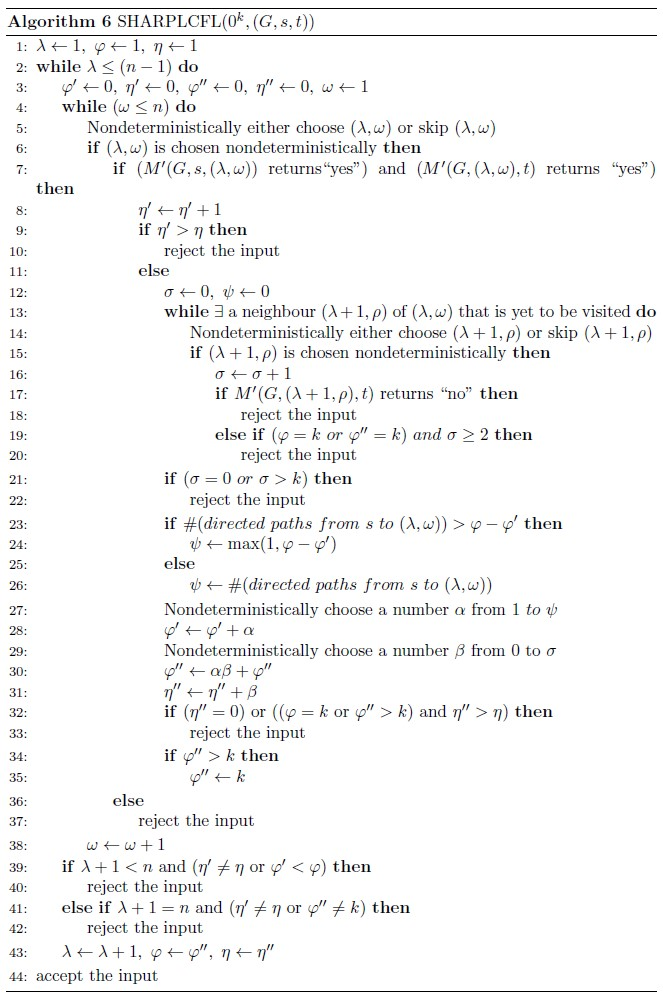
\includegraphics[scale=0.85]{Algo6-sharplcfl.jpg}\end{center}
\end{figure}

We note the following points about the SHARPLCFL algorithm.

Always $1\leq\lambda\leq n$ and $1\leq \omega\leq n$. In the {\rm SHARPLCFL} algorithm, if we choose a vertex nondeterministically we verify if it is in a directed path from $s$ to $t$ in lines 7 and 17.

The variable $\eta '$ is the number of vertices we are choosing nondeterministically in row $\lambda$ and it must be equal to $\eta$ after we have made nondeterministic choices on all the vertices in row $\lambda$ failing which we reject the input in lines 39-42. $\varphi '$ is used to verify if the number of distinct directed paths from $s$ to $t$ that pass through $\eta '$ vertices chosen nondeterministically in row $\lambda$ is atleast $\varphi$ failing which we reject the input in lines 39-40.

The variable $\sigma$ computed in line 16 inside the while loop from line 13 to 20 is the number of vertices chosen nondeterministically as the neighbours of $(\lambda ,\omega)$ in row $\lambda +1$ such that these vertices are in at least one directed path from $s$ to $t$ in $G$. Here $1\leq \sigma\leq n$.

We compute $\psi$ in lines 24 and 26 in $\FUL$ by Corollary \ref{ldag-st-subgraph-ul} without altering the number of accepting computation paths. Note that $\psi\geq 1$ since $(\lambda ,\omega)$ is in at least one directed path from $s$ to $t$ in $G$. After lines 24 and 26, $\psi$ is either ${\rm max(}1,\varphi -\varphi ')$ or {\rm \#(}directed paths from $s$ to $(\lambda ,\omega )${\rm )}. Therefore $1\leq\psi\leq\varphi$ always. From lines 1, 32-33 and 43 it follows that $1\leq \varphi\leq k$ always and so in line 30 we always have $\varphi ''\leq kn+\varphi ''\leq 2kn^2$. $1\leq \alpha\leq \psi$ and so $0\leq \varphi'\leq 2kn$ always. Also $0\leq \varphi ''\leq k$ in line 4 at the begining of the while loop. Therefore $0\leq\varphi ''\leq 2kn^2$ always.

Always $0\leq \beta\leq \sigma$, $0\leq \eta '\leq n$, $0\leq \eta ''\leq n^2$ and $1\leq \eta\leq n^2$. If $\eta >n$ then we reject the input due to the condition in lines 39 and 41.  Variables $\varphi ',~\eta '$ and $\eta ''$ are updated in the while loop from line 4 to 38 and these values do not decrease inside this loop.

Using nondeterminism to increment $\eta ''$ in lines 29 and 31 by $\beta$ is to nondeterministically avoid the possibility of counting vertices in row $\lambda +1$ that are common neighbours of two distinct vertices in row $\lambda$ more than once.

In lines 27 and 29, assume that we are always nondeterministically choosing the correct value of $\alpha $ and $\beta$ respectively in the algorithm. Then our algorithm proceeds correctly and ends in an accepting configuration if and only if we have nondeterministically chosen exactly $k$ distinct directed paths from $s$ to $t$ in $G$. On the contrary if $\varphi ''$ is updated with an incorrect value of $\alpha$ or if $\eta ''$ is incremented by an incorrect value of $\beta$, then in those iterations of the while loop from line 4 to 38, the algorithm proceeds by assuming that an alternate set of nondeterministic choices have been made on vertices in row $\lambda +1$ which agree with $\eta ''$ and $\varphi ''$.

Any two directed paths formed by nondeterministically choosing two different vertices in row $\lambda$ in lines 5-6 are distinct irrespective of their neighbours nondeterministically chosen in the row $\lambda +1$ in lines 14-15. As a result if the number of directed paths from $s$ to $t$ in $G$ is lesser than $k$ then the value of $\varphi ''$ computed in line 30 is always lesser than $k$ and these inputs are rejected in lines 41-42.

At the end of the while loop in line 38, $\varphi ''$ is the number of directed paths from $s$ to $t$ computed nondeterministically, that we need for subsequent stages of our algorithm. Also $\eta ''$ is the number of distinct vertices that are in row $\lambda +1$ in $\varphi ''$ distinct directed paths from $s$ to $t$ in $G$ which is also computed nondeterministically.

Now assume that the number of directed paths from $s$ to $t$ in $G$ is at least $k$. The cases where we reject the input since the nondeterministic choices made on the neighbours of $(\lambda ,\omega)$ in row $\lambda +1$ results in increasing the number of distinct directed paths nondeterministically chosen to be greater than $k$ is in lines 19, 20, 32 and 33.

Lines 19 and 20 are pertaining to the case when we are in vertex $(\lambda ,\omega)$ in row $\lambda$ and we are visiting the neighbours of $(\lambda ,\omega)$ in row $\lambda +1$. In this case we have already nondeterministically chosen $k$ distinct directed paths from $s$ to $t$ and we have also chosen vertices in row $\lambda +1$ in excess that results in increasing the number of distinct directed paths chosen nondeterministically from $s$ to $t$ to be greater than $k$. Similarly in lines 32 and 33 we have the case when we have chosen a $(\lambda ,\omega )$ in row $\lambda$ and we have visited all the neighbours of $(\lambda ,\omega )$ in row $\lambda +1$. If {\rm (}$\varphi =k$ or $\varphi ''>k${\rm )} and $\eta ''>\eta$ then it implies that we have chosen more than $k$ distinct directed paths from $s$ to $t$ in $G$ that most recently includes directed paths that pass through $(\lambda ,\omega$) and $\eta ''$ distinct neighbours of $(\lambda ,\omega)$ in row $\lambda +1$ and so in lines 32 and 33 we reject the input.

The case when we reject the input since we have not chosen $\eta$ vertices in row $\lambda <n-1$ or at least $\varphi$ distinct directed paths till row $\lambda <n-1$ is in lines 39 and 40. The case when we reject the input since we have not chosen exactly $k$ distinct directed paths from $s$ to $t$ but we have moved till row $n-1$ is in lines 41 and 42.

In the SHARPLCFL algorithm, since we keep track of only a constant number of variables all of which take non-negative integer values and the values of these variables are upper bounded by a polynomial in the size of the graph $G$, which is once again polynomial in the input size $|x|$ we get a $\NL$ machine that executes the SHARPLCFL algorithm. Since we have assumed that $\NL =\UL$ and we use $M'$ to verify if there exists a directed path from a vertex $s'$ to a vertex $t'$ in lines 13 and 23, it follows that the number of accepting computation paths of the $\NL$ machine described by our SHARPLCFL algorithm does not get altered upon simulating $M'$ (also see Note \ref{st-subgraph}). As a result it follows that the $\NL$ machine described by the SHARPLCFL algorithm stops in an accepting state if and only if we start from vertex $s$ in row $1$ and reach vertex $t$ in row $n$ via exactly $k$ distinct directed paths. Now as mentioned in Corollary \ref{parsicomplete}, since $f(x)$ is
  equal to the number of directed paths from $s$ to $t$ in $G$ and since we have assumed $\NL =\UL$, it
  follows that the number of accepting computation paths of this $\NL$ machine is ${{f(x)}\choose{k}}$. When $f(x)<k$ this $\NL$ machine has no
  accepting computation paths and so we get ${{f(x)}\choose {k}}=0$.
 This shows that ${{f(x)}\choose{k}}\in \sharpL$.
\end{proof}
\section{Characterization of \textrm{\boldModL}}
In this section we study the complexity class $\ModL$ and obtain a characterization of $\ModL$ that shows that a $\sharpL$ function $f$ and a $\FL$ function $g$ that outputs a prime number in unary representation are
sufficient to decide if a given input $x$ is in a language $L\in
\ModL$, however under the assumption that $\NL =\UL$. More precisely we are able to show a characterization of $\ModL$ in Theorem \ref{modlprime} that if we assume $\NL =\UL$ and we have a language $L\subseteq\Sigma^{*}$ with $L\in\ModL$ then we can decide whether an input $x\in\Sigma^{*}$ is in $L$ using $f\in\sharpL$ and $g\in\FL$ where $g(x)$ is a prime number $p$ that is output by $g$ in the unary representation such that if $x\in L$ then $f(x)\equiv 1(\mod p)$ and if $x\not\in L$ then $f(x)\equiv 0(\mod p)$. As an immediate consequence of Theorem \ref{modlprime}, %, assuming $\NL =\UL$ we
%are able to show that $\ModL$ is the logspace analogue of the
%complexity class $\ModP$. As another corollary 
we show that $\ModL$ is closed under complement assuming $\NL =\UL$ in Corollary \ref{modlcomplement}.
\begin{lemma}\label{gapltosharpl}
  Let $L\in \ModL$. Then there exists a function $f\in \sharpL$ and a
  function $g\in \FL$ such that on any input string $x$,
  \begin{itemize}
  \item $g(x)=0^{p^e}$ for some prime $p$ and a positive integer $e$,
    and
  \item $x\in L$ if and only if $f(x)\not \equiv 0(\mod p^e)$.
  \end{itemize}
\end{lemma}
\begin{proof}
  Let $L\in \ModL$ be witnessed by functions $f'\in \GapL$ and $g\in
  \FL$ as in Definition \ref{modldefn}. Now given $f'\in \GapL$ there exists
  $f_1,f_2\in \sharpL$ such that on any input string $x$ we have
  $f'(x)=f_1(x)-f_2(x)$. Consider $f(x)=f_1(x)+(p^e-1)f_2(x)$. Since
  $\sharpL$ is closed under multiplication by a $\FL$ function that
  outputs a positive integer and also under addition, we have $f(x)\in \sharpL$. Moreover on a given
  input $x$, we have $f'(x)\not \equiv 0(\mod p^e)$ if and only if
  $f'(x)=f_1(x)-f_2(x)\not \equiv 0(\mod p^e)$ if and only if
  $f(x)=f_1(x)+(p^e-1)f_2(x)\not \equiv 0(\mod p^e)$. As a result we
  can replace the $\GapL$ function $f'$ by the $\sharpL$ function $f$
  to decide if any given input string $x$ is in $L$.
\end{proof}

\begin{theorem}\label{modlprime}
  Assume that $\NL =\UL$ and let $L\in \ModL$. Then there exists a
  function $f\in \sharpL$ and a function $g\in \FL$ such that on any
  input string $x$,
  \begin{itemize}
  \item $g(x)=0^p$ for some prime $p>0$, and,
  \item if $x\in L$ then $f(x)\equiv 1(\mod p)$,
  \item if $x\not\in L$ then $f(x)\equiv 0(\mod p)$.
  \end{itemize}
\end{theorem}

\begin{proof}
  Let $L\in \ModL$. It follows from Lemma \ref{gapltosharpl} that
  there exists $f'\in \sharpL$ and $g'\in \FL$ such that on any input
  string $x$ we have $g'(x)=0^{p^e}$ for some prime $p$ and a positive
  integer $e$, and $x\in L$ if and only if $f'(x)\not \equiv 0(\mod
  p^e)$. Let $g$ be a $\FL$ function that outputs the prime $p$ in unary when
  given the input $x$. Now assume that there exists a $f''\in \sharpL$
  such that $f'(x)\not \equiv 0(\mod p^e)$ if and only if $f''(x)\not
  \equiv 0(\mod p)$. Then $x\in L$ if and only if $f''(x)\not \equiv
  0(\mod p)$. Define $f(x)=(f''(x))^{(p-1)}$. Using Fermat's Little
  Theorem we have, if $x\in L$ then $f(x)\equiv 1(\mod
  p)$. Otherwise if $x\not \in L$ then $f(x)\equiv 0(\mod p)$. We
  therefore prove the theorem statement if we define the function
  $f''$ such that $f'(x)\not \equiv 0(\mod p^e)$ if and only if
  $f''(x)\not \equiv 0(\mod p)$.

  It is easy to see that we can compute the largest power of $p$ that
  divides $p^e=|g'(x)|$ in $\FL$. If $e=1$ then we define $f''=f'$
  where $f'$ is the $\sharpL$ function in Lemma \ref{gapltosharpl}. It
  is clear that on an input string $x$ we have $g(x)=g'(x)=0^p$ for
  some prime $p$ and $x\in L$ if and only if $f'(x)\not \equiv 0(\mod
  p^e)$ which is true if and only if $f''(x)\not \equiv 0(\mod p)$. Otherwise $e\geq 2$. Here we have $g'(x)=0^{p^e}$ and $g(x)=0^p$. Now we use induction on
  $(e-1)$ to define $f''$. Inductively assume that for $1\leq i\leq
  (e-1)$ we have functions $f_i\in \sharpL$ such that $f'(x)\not
  \equiv 0(\mod p^i)$ if and only if $f_i(x)\not \equiv 0(\mod
  p)$. For the case when $(e-1)=1$ we can have $f_{e-1}=f'$. Then it
  is clear that given an input string $x$, we have $f'(x)$ is
  divisible by $p^e$ if and only if
  \begin{enumerate}
  \item $f'(x)$ is divisible by $p^{e-1}$, and
  \item \label{condition2}the coefficient of $p^{e-1}$ in the base-$p$
    expansion of $f'(x)$ is zero.
  \end{enumerate}
  Here Condition \ref{condition2} stated above is equivalent to
  ${{f'(x)}\choose{p^{e-1}}}\equiv 0(\mod p)$. Therefore $f'(x)\not \equiv 0(\mod p^e)$ if and only if
  $\{ f'(x)\not \equiv 0(\mod p^{e-1})$ or
  ${{f'(x)}\choose{p^{e-1}}}\not \equiv 0(\mod p)\}$ which is true if
  and only if $\{ f_{e-1}(x)\not \equiv 0(\mod p)$ or
  ${{f'(x)}\choose{p^{e-1}}}\not \equiv 0(\mod p)\}$. Let $f_e'(x)=(f_{e-1}(x))^{p-1}{{f'(x)}\choose{p^{e-1}}}^{p-1}+((f_{e-1}(x))^{p-1}+p-1){{f'(x)}\choose{p^{e-1}}}^{p-1}+(f_{e-1}(x))^{p-1}({{f'(x)}\choose{p^{e-1}}}^{p-1}+(p-1))$. Now define $f_e(x)=(f_e'(x))^{p-1}$. Using
  Theorem \ref{sharplchoosefl} and closure properties of $\sharpL$ it
  follows that $f_e\in \sharpL$. Moreover on an input $x$, if $f'(x)\equiv 0(\mod p^e)$ then $f_e(x)\equiv 0(\mod p)$. On the other hand if $f'(x)\not\equiv 0(\mod p^e)$ then we consider the following cases. Case 1: $f'(x)\equiv 0(\mod p^{e-1})$: Then $f_{e-1}(x)\equiv 0(\mod p)$ and we also have ${{f'(x)}\choose{p^{e-1}}}\not\equiv 0(\mod p)$. As a result from the definition of $f_e(x)$ we get $f_e(x)\equiv 1(\mod p)$.\newline
Case 2: $f'(x)\not\equiv 0(\mod p^{e-1})$: Then $f_{e-1}(x)\not \equiv 0(\mod p)$ and we can have either ${{f'(x)}\choose{p^{e-1}}}\not\equiv 0(\mod p)$ or ${{f'(x)}\choose{p^{e-1}}}\equiv 0(\mod p)$. But in both of these cases we get $f_e(x)\equiv 1(\mod p)$. As a result defining $f''=f_e$ we complete the proof.
\end{proof}

%\begin{corollary}
% Assume that $\NL =\UL$. Then $\ModL$ is the logspace analogue of $\ModP$.
%\end{corollary}

\begin{corollary}\label{modlcomplement}
  Assume that $\NL =\UL$. Then $\ModL$ is closed under complement.
\end{corollary}

\begin{proof}
  Let $L\in \ModL$. Then by Theorem \ref{modlprime} there exists $f
  \in \sharpL$ and $g\in \FL$ such that on any input $x$, we have
  $g(x)=0^p$ for some prime $p$ and if $x\in L$ then $f(x)\equiv
  1(\mod p)$. Otherwise if $x\not\in L$ then $f(x)\equiv 0(\mod p)$.

  Let $h(x)=(f(x)+(p-1))^{(p-1)}$. Using closure properties of $\sharpL$ it follows that $h(x)\in \sharpL$. Using Fermat's Little
  Theorem we have, if $x\in L$ then $h(x)\equiv 0(\mod
  p)$ and if $x\not\in L$ then $h(x)\equiv 1(\mod p)$. Clearly this
  shows $\overline{L}\in \ModL$ or that $\ModL$ is closed under
  complement.
\end{proof}

\section{Closure properties of $\boldModL$}\label{chap04-closureModL}
As a consequence of the characterization of $\ModL$ that we have shown in Theorem \ref{modlprime}, it is shown in Corollary \ref{modlcomplement} that $\ModL$ is closed under complement under the assumption that $\NL =\UL$. We continue to study the complexity class $\ModL$ and obtain its closure properties which follow due to the above stated characterization of $\ModL$.
\subsection{An unconditional closure property of \textrm{ModL}}
\begin{definition}
Let $\Sigma$ be the input alphabet such that $\{ 0,1\}\subseteq\Sigma$ and let $L_1,L_2\subseteq\Sigma ^{*}$. We define the join of $L_1$ and $L_2$ to be $L_1\vee L_2=\{ x1|x\in L_1\}\cup \{ y0|y\in L_2\}$.
\end{definition}
\begin{theorem}\label{modljoin}
If $\{ 0,1\}\subseteq\Sigma$ and $L_1\in\ModL$ then $L_1\vee L_2\in\ModL$.
\end{theorem}
\begin{proof}
Let $L_i\in \ModL$ and assume that we decide if an input string $x\in\Sigma^{*}$ is in $L_i$ using functions  $f_i\in\GapL$ and $g_i\in \FL$ where $1\leq i\leq 2$ respectively. We assume without loss of generality that the size of any  input string $x$ is at least $1$. Let $x=x_1x_2\cdots x_{n+1}$ and let $y=x_1\cdots x_n$ where $n\in\Z^{+}$. Also let 
\[ f(x)=\left \{ \begin{array}{ll}
	f_1(y) & \mbox{if $x_{n+1}=1$}\\
	f_2(y) & \mbox{otherwise if $x_{n+1}=0$,}
\end{array}
\right. \]
and
\[ g(x)=\left \{ \begin{array}{ll}
	g_1(y) & \mbox{if $x_{n+1}=1$}\\
	g_2(y) & \mbox{otherwise if $x_{n+1}=0$.}
\end{array}
\right. \]
It is easy to note that $f\in\GapL$ and $g\in\FL$. Since $|g_1(x)|$ or $|g_2(x)|$ is always a prime power on any input string $x\in\Sigma ^{*}$ it follows that $|g(x)|$ is also a prime power. Now $f(x)\not\equiv 0(\mod |g(x)|)$ for any input $x=yx_{n+1}$ if and only if exactly one of the following is true:
($x_{n+1}=1$ and $y\in L_1$) or ($x_{n+1}=0$ and $y\in L_2$). Clearly this shows that $L_1\vee L_2\in\ModL$ and that we can decide if any input string $x\in\Sigma ^{*}$ is in $L_1\vee L_2$ using $f\in\GapL$ and $g\in\FL$ which completes the proof.
\end{proof}
In Theorem \ref{modlunconclos}(\ref{modlmany}) we show that $\ModL$ is closed under $\leq ^{\L}_m$ reductions and similarly in Theorem \ref{modlunconclos}(\ref{modlulmany}) we show that $\ModL$ is closed under $\leq ^{\ULredn}_m$ reductions. Using Theorem \ref{modlprime} and Corollary \ref{modlcomplement} we show in Theorem \ref{modlconclos}(\ref{modl1trt}) that $\ModL$ is closed under $\leq ^{\L}_{1-\trt}$ reductions assuming $\NL =\UL$.  We also show that if $\NL =\UL$ then $\ModL$ is closed under $\leq ^{\ULredn}_{1-\trt}$ reductions in Theorem \ref{modlconclos}(\ref{modlul1trt}). The following table lists the closure properties of $\ModL$ that are known.
\begin{center}
\begin{tabular}{||c|c|l||}\hline\hline
\emph{Closure property} & \emph{Assumptions} & \emph{Reference} \\ \hline\hline
$\vee$ (join) & unconditional & Theorem \ref{modljoin} \\ \hline
complement & $\NL =\UL$ & Corollary \ref{modlcomplement} \\ \hline
${\Lredn}$ & unconditional & Theorem \ref{modlunconclos}(\ref{modlmany}) \\ \hline
$\leq^{\ULredn}_m$ & unconditional & Theorem \ref{modlunconclos}(\ref{modlulmany}) \\ \hline
$\leq_{1-\trt}^{\L}$ & $\NL =\UL$ & Theorem \ref{modlconclos}(\ref{modl1trt}) \\ \hline
$\leq^{\ULredn}_{1-\trt}$ & $\NL =\UL$ & Theorem \ref{modlconclos}(\ref{modlul1trt}) \\ \hline\hline
\end{tabular}
\end{center}
\begin{center}Table 1: Closure properties of $\ModL$\end{center}
We also show that $\ModL^{\ULredn}=\ModL$ assuming $\UL =\coUL$ in Theorem \ref{modlulT}. As a consequence of these results we show in Corollary \ref{modlulmodl} that $\UL_{1-\trt}^{\ModLredn}=\ModL^{\ULredn}=\ModL$ assuming $\NL =\UL$.

\section{Reducibilities of $\boldModL$}\label{modl-closure-properties}
We recall the definitions stated in Section \ref{Chap01-Sec-Reduceoracle} of Chapter 1.
\subsection{Reducibilities}
\begin{definition}
Let $\Sigma$ be the input alphabet and let $L_1,L_2\subseteq\Sigma^{*}$. We say that $L_1$ is logspace conjunctive truth-table reducible to $L_2$, denoted by $L_1\leq ^{\L}_{\ctt}L_2$, if there exists $f\in\FL$ such that given an input $x\in\Sigma ^{*}$ of length $n$ we have $f\in\FL$ such that $f(x)=\{ y_1\ldots ,y_{p(n)}\}$ and $x\in L_1$ if and only if $y_i\in L_2$ for every $1\leq i\leq p(n)$ where $p(n)$ is a polynomial in $n$.
\end{definition}
\begin{definition}
Let $\Sigma$ be the input alphabet and let $L_1,L_2\subseteq\Sigma^{*}$. We say that $L_1$ is logspace $k$-conjunctive truth-table reducible to $L_2$, denoted by $L_1\leq ^{\L}_{k-\ctt}L_2$, if there exists $f\in\FL$ such that given an input $x\in\Sigma ^{*}$ of length $n$ $f(x)=\{ y_1\ldots ,y_k\}$ and $x\in L_1$ if and only if $y_i\in L_2$ for every $1\leq i\leq k$.
\end{definition}
\begin{definition}
Let $\Sigma$ be the input alphabet and let $L_1,L_2\subseteq\Sigma^{*}$. We say that $L_1$ is logspace disjunctive truth-table reducible to $L_2$, denoted by $L_1\leq ^{\L}_{\dtt}L_2$, if there exists $f\in\FL$ such that given an input $x\in\Sigma ^{*}$ of length $n$ we have $f(x)=\{ y_1,\ldots ,y_{p(n)}\}$ and $x\in L_1$ if and only if $y_i\in L_2$ for at least one $1\leq i\leq p(n)$ where $p(n)$ is a polynomial in $n$.
\end{definition}
\begin{definition}
Let $\Sigma$ be the input alphabet and let $L_1,L_2\subseteq\Sigma^{*}$. We say that $L_1$ is logspace $k$-disjunctive truth-table reducible to $L_2$ for some $k\in\Z^{+}$, $k\geq 1$, denoted by $L_1\leq ^{\L}_{k-\dtt}L_2$, if there exists  $f\in\FL$ such that given an input $x\in\Sigma ^{*}$ of length $n$ we have $f(x)=\{ y_1,\ldots ,y_k\}$ and $x\in L_1$ if and only if $y_i\in L_2$ for at least one $1\leq i\leq k$.
\end{definition}
\begin{definition}\label{logspace1ttdefn}
Let $\Sigma$ be the input alphabet and let $L_1,L_2\subseteq\Sigma ^{*}$. We say that $L_1$ is logspace $1$-truth-table reducible to $L_2$ and denoted by $L_1\leq^{\L}_{1-\trt}L_2$ if there exists a $O(\log n)$ space bounded Turing machine $M^{L_2}$ that has access to $L_2$ as an oracle such that $M^{L_2}$ decides if any given input $x\in\Sigma^{*}$ is in $L_1$ by making exactly one query to the oracle $L_2$, where $n=|x|$.
\end{definition}
\begin{definition}\label{ulmanyonedefn}
Let $\Sigma$ be the input alphabet and let $L_1,L_2\subseteq\Sigma ^{*}$. We say that $L_1\leq ^{\ULredn}_mL_2$ if there exists a $\FNL$ Turing machine $M$ such that on any input $x\in\Sigma ^{*}$ the number of accepting computation paths of $M(x)$ is at most $1$. Also if $x\in L_1$ then there exists an accepting computation path of $M$ on input $x$ such that if we obtain $y\in\Sigma^{*}$ as the output along the accepting computation path then $y\in L_2$. If $x\not\in L_1$ then either $M$ does not have any accepting computation path on input $x$ or if there exists an accepting computation path of $M$ on input $x$ and $y\in\Sigma^{*}$ is the output along this computation path then $y\not\in L_2$.
\end{definition}
\begin{definition}\label{ul1ttdefn}
Let $\Sigma$ be the input alphabet and let $L_1,L_2\subseteq\Sigma ^{*}$. We say that $L_1\leq ^{\ULredn}_{1-\trt}L_2$ if there exists a $\NL$ machine $M^{L_2}$ with access to the oracle $L_2$ such that on any input $x\in\Sigma ^{*}$ the number of accepting computation paths of $M^{L_2}(x)$ is at most $1$. Also $M^{L_2}$ submits exactly one query $q_x\in\Sigma^{*}$ to the $L_2$ oracle on any input $x\in\Sigma^{*}$ to decide if $x\in L_1$.  We assume that the query is submitted by the $\NL$ machine $M^{L_2}$ in a deterministic manner to the $L_2$ oracle according to the Ruzzo-Simon-Tompa oracle access mechanism stated above. Here if $x\in L_1$ then there exists exactly one accepting computation path of $M^{L_2}$ on input $x$. Otherwise if $x\not\in L_1$ then $M^{L_2}$ rejects the input $x$ on all of its computation paths.
\end{definition}

\subsection{\textrm{ModL}}

We recall the definiton of $\ModL$ stated in Definition \ref{modldefn}.
\begin{definition}
Let $\Sigma$ be the input alphabet and let $A\in\Sigma^*$. We define the complexity class $\ModL^A$ to be the class of all languages $L\in\Sigma^*$ for which there exists a $\NL$ machine $M^A$ with access to the oracle $A$ and a function $g\in\FL$ such that on any input $x\in\Sigma^*$ if $f(x)=\gap_{M^A}(x)$, we have
\begin{itemize}
\item $g(x)=1^{p^e}$ for some prime $p$ and a positive integer $e$, and
\item $x\in L\Leftrightarrow f(x)\not \equiv 0(\mod p^e)$.
\end{itemize}
Here the $\NL$ machine $M^A$ submits queries to the oracle $A$ in a deterministic manner according to the Ruzzo-Simon-Tompa oracle access mechanism stated above. Along any computation path the $\NL$ machine $M^A$ ends in an accepting state or in a rejecting state depending on the input $x$ and the replies given by the oracle $A$.
\end{definition}
\begin{definition}
Let $\Sigma$ be the input alphabet and let $L_1,L_2\in \Sigma ^*$. We define the complexity class $\UL^{\small \ModL}_{1-\trt}=\{L_1|L_1\leq ^{\ULredn}_{1-\trt}L_2$, where $L_2\in\ModL\}$.
\end{definition}
\begin{definition}\label{modluldefn}
Let $\Sigma$ be the input alphabet and let $L_1,L_2\in \Sigma ^*$. We define the complexity class $\ModL^{\small \UL}=\{L_1|L_1\in \ModL^{L_2}$, where $L_2\in\ModL\}$.
\end{definition}

\begin{lemma}\label{fillacceptpaths}
Let $\Sigma$ be the input alphabet and let $g\in \FL$ such that on any input $x\in \Sigma ^*$, we have $g(x)$ to be a prime number $p$ in the unary notation that depends on the input $x$. Then there exists a $\NL$ machine $M$ such that the lexicographically least $|g(x)|$ computation paths are exactly the only accepting computation paths in the computation tree of $M$.
\end{lemma}
\begin{proof}
Let $x\in\Sigma^*$ such that $n=|x|$ and let $g(x)=0^p$ for some prime $p\in\Z^+$. Let $k\in\Z^+$ such that $2^{k-1}\leq p<2^k$. It is easy to see that $k,p\in O(\log n)$. The $\NL$ machine $M$ simulates $g$ on input $x$ and computes $p=|g(x)|$. The $\NL$ machine $M$ then non-deterministically makes $k$ choices and accepts in a computation path if the non-deterministic choices are a binary string less than or equal to $p$. $M$ rejects along all other computation paths.
\end{proof}

Apart from the chararacterization of $\ModL$ shown in Theorem \ref{modlprime}, we also need Lemma \ref{gapltosharpl}.

\begin{theorem}\label{modlunconclos}
Let $\Sigma$ be the input alphabet and let $L_1,L_2\subseteq \Sigma ^{*}$. Also let $L_2\in\ModL$. Now 
\begin{enumerate}
\item\label{modlmany} if $L_1{\Lredn} L_2$ then $L_1\in\ModL$, and
\item\label{modlulmany} if $L_1\leq^{\ULredn}_mL_2$ then $L_1\in\ModL$.
\end{enumerate}
\end{theorem}
\begin{proof}
\begin{enumerate}
\item Let $L_2\in\ModL$ and let $f_2\in\GapL$ and $g_2\in\FL$ be functions using which we decide if an input $x\in\Sigma ^{*}$ is in $L_2$. Also let $L_1\leq ^{\Lredn}_mL_2$ using $f\in\FL$. If $x\in\Sigma^{*}$ is the input then $x\in L_1$ if and only if $f(x)\in L_2$. But $L_2\in\ModL$ and therefore $f(x)\in L_2$ if and only if $f_2(f(x))\not\equiv 0(\mod p^e)$ where $p^e=|g_2(f(x))|\in\Z^{+}$ where $p,e\in\Z^{+}$ with $p$ being a prime and $e\geq 1$. Now it is easy to note that $(f_2\circ f)\in\GapL$ and $(g_2\circ f)\in\FL$. Clearly $g_2(f(x))$ is a prime power in the unary representation for any $x\in\Sigma ^{*}$. As a result if $x\in\Sigma ^{*}$ then $x\in L_1$ if and only if $f_2(f(x))\not\equiv 0(\mod p^e)$ where $p^e=|g_2(f(x))|$ which shows $L_1\in\ModL$.

\item We recall the definition $\leq^{\ULredn}_m$ from Definition \ref{ulmanyonedefn}. The proof of this assertion is similar to Theorem \ref{modlunconclos}(\ref{modlmany}). We use Lemma \ref{gapltosharpl} for $L_2\in \ModL$ and assume that there exists $f\in\sharpL$ and $g\in\FL$ such that on any input $x\in\Sigma^{*}$ we have $g(x)=1^{p^e}$ where $p,e\in\Z^{+}$, $p$ is a prime, $e\geq 1$ and $x\in L_2$ if and only if $f(x)\not\equiv 0(\mod p^e)$. We know that the $\leq^{\ULredn}_m$ reduction has at most one accepting computation path. Therefore if the computation path we obtain is an accepting computation path and $y\in\Sigma^{*}$ is output along this accepting computation path, then simulating the $\NL$ machine for $L_2\in\ModL$ with $y$ as the input shows that the congruence relation based on the $\sharpL$ function $f$ and the $\FL$ function $g$ that is used to decide if any input $x\in\Sigma ^{*}$ is in $L_2$ can also be used for deciding if $x\in L_1$. Otherwise if the computation path of the $\leq^{\ULredn}_m$ reduction that we obtain is a rejecting computation path then using Lemma \ref{fillacceptpaths} it follows that our $\NL$ machine can make sufficiently many non-deterministic choices so that the number of accepting computation paths that we obtain at the end of each of these rejecting computation paths is divisible by $|g(x)|$. This shows $L_1\in\ModL$.
\end{enumerate}
\end{proof}

\begin{theorem}\label{modlconclos}
Let $\Sigma$ be the input alphabet and let $L_1,L_2\subseteq \Sigma ^{*}$. Also let $L_2\in\ModL$ and assume that $\NL =\UL$. Now
\begin{enumerate}
\item \label{modl1trt} if $L_1\leq ^{\mathrm{L}}_{1-\trt}L_2$ then $L_1\in\ModL$, and 
\item \label{modlul1trt} if $L_1\leq^{\ULredn}_{1-\trt}L_2$ then $L_1\in\ModL$.
\end{enumerate}
\end{theorem}
\begin{proof}
\begin{enumerate}
\item We recall the definition of $\leq^{\Lredn}_{1-\trt}$ from Definition \ref{logspace1ttdefn}. Let $L_1\leq ^{\Lredn}_{1-\trt}L_2$ using $f\in\FL$ that makes exactly one query to the oracle $L_2$. In other words, $f$ correctly decides if an input $x\in\Sigma^{*}$ is in $L_1$ by making exactly one query to the oracle $L_2$. Also let  $q_x\in\Sigma ^{*}$ be the query string that is generated by $f$ for the input $x\in\Sigma ^{*}$. Clearly $f$ decides if $x\in L_1$ based on $x$ and the reply of the oracle $L_2$ when the oracle $L_2$ is given the query $q_x$ as input. Therefore let $f'\in\FL$ be the function that generates and outputs the query $q_x$ generated by $f$ when it is given the input $x$. Also let $g'\in\FL$ be such that $g'(x,\chi _{L_2}(q_x))=f(x)$ where $\chi _{L_2}$ is the characteristic function of $L_2$. It is clear that $g'$ correctly decides whether any input $x\in L_1$ if the reply of the oracle $L_2$ is also given to it.

Since $L_2\in\ModL$ and we have assumed $\NL =\UL$, it follows from Theorem \ref{modlprime} that there exists $f_2\in\sharpL$ and $g_2\in\FL$ such that on any input $x\in\Sigma^{*}$ we have if $x\in L_2$ then $f_2(x)\equiv 1(\mod p)$ and if $x\not \in L_2$ then $f_2(x)\equiv 0(\mod p)$, where $g_2(x)=1^p$, $p\in\Z^{+}$ and $p$ is a prime. Let us consider the function $(g_2\circ f')$. Given an input $x\in \Sigma^*$, $g_2(f(x))=1^p$, for some prime $p\in\Z^+$ which depends on the query $f'(x)$ generated from the input $x$. It is clear that $(g_2\circ f')\in\FL$. Consider the function $(g'\circ f_2\circ f')$ and let $M$ denote the $\NL$ machine corresponding to it. The $\NL$ machine $M$ considers the output of a computation path of the $\NL$ machine corresponding to $(f_2\circ f')(x)$ as $\chi _{L_2}(q_x)$. Since $g'\in\FL$ it follows that the output of $M$ is the same along all the accepting computation paths of the $\NL$ machine corresponding to $(f_2\circ f')$. In other words, either $M$ accepts along all the accepting computation paths of the $\NL$ machine corresponding to $(f_2\circ f')$ or $M$ rejects along all the accepting computation paths of the $\NL$ machine corresponding to $(f_2\circ f')$. Similarly either $M$ accepts along all the rejecting computation paths of the $\NL$ machine corresponding to $(f_2\circ f')$ or $M$ rejects along all the rejecting computation paths of the $\NL$ machine corresponding to $(f_2\circ f')$.

Let $x\in\Sigma^{*}$ be the input and let $g_2(f'(x))=1^p$. We now define a $\NL$ machine $M'$ that makes $(p-1)$ simulations of $M$ on the input $x$. In addition $M'$ also stores if the computation path chosen is the lexicographically least in its computation tree on any input $x\in\Sigma^{*}$. Now if the output of $M$ along any of its computation paths is the same as the output of the computation path of the $\NL$ machine corresponding to $(f_2\circ f')$ on the input $x$ then $M'$ makes $(p-1)$ times the simulation of $M$ on input $x$ and stops. In this case, for a given input $x\in\Sigma^{*}$, if $L_1\leq ^{\mathrm{L}}_{1-\trt}L_2$ then along every computation path the reduction is similar to a logspace many-one reduction from $L_1$ to $L_2$. In this case using Fermat's Little Theorem, it follows from our observations that if $x\in L_1$ then $\acc _{M'}(x)\equiv 1(\mod p)$ and if $x\not \in L_1$ then $\acc _{M'}(x)\equiv 0(\mod p)$. This shows $L_1\in\ModL$. On the other hand if we have the output of $M$ along any of its computation paths is the complement of the output of the computation path of the $\NL$ machine corresponding to $(f_2\circ f')$ on a given input $x\in\Sigma^{*}$ then also $M'$ makes $(p-1)$ simulations of $M$ on input $x$. However in these $(p-1)$ simulations of $M$ by $M'$, along any of the computation paths of $M'$ that is not the lexicographically least computation path we assume that $M'$ stops with the output of $M$ on input $x$. Along the lexicographically least computation path that we obtain in these $(p-1)$ simulations of $M$ by $M'$ we assume that $M'$ makes sufficiently many non-deterministic choices at the end of this computation path as in Lemma \ref{fillacceptpaths} so that we obtain $\acc _{M'}(x)=\acc _M(x)^{p-1}+(p-1)$. In this case using Fermat's Little Theorem, it follows from our observations that if $x\in L_1$ then $\acc _{M'}(x)\equiv 0(\mod p)$ and if $x\not \in L_1$ then $\acc _{M'}(x)\not\equiv 0(\mod p)$ which implies $\overline{L_1}\in \ModL$. We now use our assumption that $\NL=\UL$ and so it follows from Corollary \ref{modlcomplement} that $L_1\in\ModL$ and this completes the proof.

\item We recall the definition of $\leq^{\ULredn}_{1-\trt}$ from Definition \ref{ul1ttdefn}. We follow the Ruzzo-Simon-Tompa oracle access mechanism stated in Section \ref{chap1-NOTM} and generate the query string $q_x\in\Sigma^*$ given the input $x\in\Sigma^*$ in a deterministic manner using $O(\log n)$ space. Our proof follows from our assumption that $\NL=\UL$ and a case analysis similar to the proof of Theorem \ref{modlconclos}(\ref{modl1trt}) depending on whether the $\leq^{\ULredn}_{1-\trt}$ reduction is similar to a $\leq^{\ULredn}_m$ reduction or if the output of the computation paths of the $\NL$ machine that is used in the reduction is the complement of the output of the computation paths of the $\NL$ machine for the oracle $L_2$ on the query string $q_x$.
\end{enumerate}
\end{proof}

\begin{theorem}\label{modlulT}
Assume that $\UL =\coUL$. Then $\ModL ^{\ULredn}\subseteq\ModL$.
\end{theorem}
\begin{proof}
The containment $\ModL\subseteq\ModL^{\ULredn}$ follows immediately from the definition of $\ModL$. To show the converse, assume that $\UL =\coUL$. Let $\Sigma$ be the input alphabet and let $L_1,L_2\subseteq\Sigma^{*}$. Also let $L_2\in\UL$ and $L_1\in\ModL^{L_2}$. As a result using Lemma \ref{gapltosharpl} for $L_1$ it follows from Definition \ref{modluldefn} that on any input $x\in\Sigma^{*}$ there exists a $\NL$ machine $M^{L_2}$ with oracle $L_2$ such that there exists $f\in\sharpL$, where $f(x)=\acc_{M^{L_2}}(x)$, and $g\in\FL$ and we have $x\in L_1$ if and only if $f(x)\not\equiv 0(\mod |g(x)|)$ where $g(x)=1^{p^e}$ with $p,e\in\Z^{+}$, $p$ being a prime and $e\geq 1$. Here we assume that the queries that are submitted to the oracle $L_2$ by $M$ are generated in a deterministic manner based on the length of the input according to the Ruzzo-Simon-Tompa oracle access mechanism stated in Section \ref{chap1-NOTM}. As a consequence we assume that $M$ submits the queries to the $L_2$ oracle and also obtains the reply of the oracle on the oracle tape before it starts any other computation on the input. In addition since $M$ is $O(\log n)$ space bounded, for any given input $x\in\Sigma^{*}$ such that $n=|x|$, it is clear that the size of each query is at most $n^j$ and the number of queries that $M$ can submit to $L_2$ is at most $n^k$ where $j,k\in\Z^{+}$. Let us denote the $i^{th}$ query that is generated by $M$ as $q_x^{(i)}\in\Sigma^{*}$ where $1\leq i\leq n^k$.

The $\NL$ machine $M'$ that we define for $L_1$ simulates $M$ on the input $x$. However unlike $M$ the $\NL$ machine $M'$ does not have access to any oracle. However $M'$ needs to obtain the reply of the $L_2$ oracle for the queries that $M$ submits in its computation path. For this purpose we assume that $M'$ generates the $i^{th}$ query $q_x^{(i)}$ in a deterministic manner during its simulation of $M$ on input $x$, where $1\leq i\leq n^k$. For every query $q_x^{(i)}$ that is generated by $M'$, to determine if $q_x^{(i)}\in L_2$, the $\NL$ machine $M'$  simulates the $\NL$ machine $M_{L_2}$ corresponding to $L_2\in \UL$. Clearly if $q_x^{(i)}\in L_2$ then $M_{L_2}$ has exactly one accepting computation path. If the simulation of $M_{L_2}$ by $M'$ results in this accepting computation path then $M'$ assumes the output of the oracle query that $M$ would have obtained when it submits the query $q_x^{(i)}$ as input to the $L_2$ oracle to be ``yes" and it continues its simulation of $M$ on input $x$. Otherwise let us assume that the simulation of $M_{L_2}$ by $M'$ results in a rejecting computation path. In this case to test if $q_x^{(i)}\in\overline{L_2}$ we use the assumption that $\UL =\coUL$ and hence allow $M'$ to simulate  the $\NL$ machine $M_{\overline{L_2}}$ for $\overline{L_2}$ (which is also a language in $\UL$) on input $q_x^{(i)}$ to test if this simulation results in an accepting computation path. If $M'$ ends in an accepting computation path in this simulation then it implies $q_x^{(i)}\in\overline{L_2}$. Therefore  $M'$ assumes that the reply of the $L_2$ oracle is ``no" on the query $q_x^{(i)}$ and continues its simulation of $M$ on input $x$. Otherwise if both these simulations of $M'$ on input $q_x^{(i)}$ results only in rejecting computation paths then $M'$ makes sufficiently many non-deterministic choices in the computation tree and ends in a rejecting state in all these computation paths. For any query string $q_x^{(i)}$ that is generated by $M'$ along any of its computation paths we either have $q_x^{(i)}\in L_2$ or we have $q_x^{(i)}\in\overline{L_2}$, where $1\leq i\leq n^k$. Now it follows from the definition of $M'$ that we can determine if $q_x^{(i)}\in L_2$ by simulating $M_{L_2}$ or if necessary $M_{\overline{L_2}}$ on $q_x^{(i)}$ during its computation on the input $x$, where $1\leq i\leq n^k$. Due to our assumption that $\UL =\coUL$ it also follows that the number of computation paths in these simulations that correctly determine if $q_x^{(i)}\in L_2$ is exactly one where $1\leq i\leq n^k$. Apart from simulating $M_{L_2}$ and $M_{\overline{L_2}}$ since the computation of $M'$ is identical to $M$ on input $x$ it follows that $\acc _{M'}(x)=f(x)$. As a result we have $x\in L_1$ if and only if $\acc_{M'}(x)\not\equiv 0(\mod |g(x)|)$. This shows $L_1\in\ModL$ due to Lemma \ref{gapltosharpl}. We therefore get $\ModL^{\ULredn}=\ModL$.
\end{proof}

\begin{corollary}\label{modlulmodl}
Assume that $\NL =\UL$. Then $\UL ^{\ModLredn}_{1-\trt}=\ModL ^{\ULredn}=\ModL$.
\end{corollary}
\begin{proof}
Since we know that $\NL$ is closed under complement from Theorem \ref{chap2-NLcomplement}, our assumption that $\NL =\UL$ implies $\UL =\coUL$. Proof of our result now follows from Theorem \ref{modlconclos}(\ref{modlul1trt}) and Theorem \ref{modlulT}.
\end{proof}

\section{Properties of the Probabilistic Logarithmic space bounded counting class ($\boldPL$)}
\begin{proposition}\label{characterizePL}
Let $\Sigma$ be the input alphabet. The class $\PL$ consists of those languages $L\subseteq\Sigma^*$ such that for some $\GapL$ function $f$ and all $x\in\Sigma^*$
\begin{itemize}
\item if $x\in L$ then $f(x)>0$
\item if $x\not\in L$ then $f(x)<0$.
\end{itemize}
\end{proposition}
\begin{proof}
For a $\GapL$ function $f$, the $\GapL$ function $2f(x)-1$ has the same sign as $f(x)$ for positive and negative values of $f(x)$ and takes value $-1$ for $f(x)=0$.
\end{proof}

\begin{corollary}\label{plclosurecomplement}
$\PL$ is closed under complement.
\end{corollary}

\begin{lemma}\label{gaplfunctionsdefine}
Define
\[\begin{array}{c}
P_n(x) = (x-1)\prod_{i=1}^n(x-2^i)^2. \\
A_n(x)=P_n(-x))^{\frac{n}{2}+1}-(P_n(x))^{\frac{n}{2}+1}. \\
B_n(x)=P_n(-x))^{\frac{n}{2}+1}+(P_n(x))^{\frac{n}{2}+1}. \\
S_n(x)=\frac{A_n}{B_n}.
\end{array}\]
Then, for $n\geq 1$,
\begin{enumerate}
\item If $1\leq x\leq 2^n$ then $0\leq 4P_n(x)<-P_n(-x)$.
\item If $1\leq x\leq 2^n$ then $1\leq S_n<\frac{5}{3}$.
\item If $-2^n\leq x\leq -1$ then $-\frac{5}{3}<S_n(x)\leq -1$.
\end{enumerate}
\end{lemma}
\begin{proof}
\begin{enumerate}
\item Since $x\geq 1$, we have that $P_n(x)\geq 0$. Clearly, $x-1<x+1$, and $(x-2^i)^2<(-x-2^i)^2$ for $i=1,\ldots ,n$. Also, if $2^{k-1}\leq x<2^k$ then $4(x-2^k)^2\leq 4.2^{2k-2}=2^{2k}<(-x-2^k)^2$. Together these imply that $4P_n(x)<-P_n(-x)$.
\item If $P_n(x)=0$ then $S_n(x)=1$. If $P_n(x)\neq 0$, then we can write
\[
S_n(x)=1+\frac{2}{\left(\left(\frac{-P_n(-x)}{P_n(x)}\right)-1\right)}.
\]
Simple algebra and part (1) yield the desired result.
\item This follows from (2) and the fact that $S_n(x)$ is an odd function, i.e., $S_n(-x)=-S_n(x)$.
\end{enumerate}
\end{proof}

\begin{theorem}\label{plclosureunion}
$\PL$ is closed under union.
\end{theorem}
\begin{proof}
Fix two languages $D$ and $E$ in $\PL$. We will show that $D\cup E$ is also in $\PL$.

Let $f_D$ and $f_E$ be the functions given by Proposition \ref{characterizePL} for $D$ and $E$, respectively. By Lemma \ref{computationpathsupperbound}, let $n=n(|x|)$ be a polynomial such that $2^n$ bounds the maximum absolute value of $f_D(x)$ and $f_E(x)$. Define $A_D(x)=A_n(f_D(x))$. Similarly, define $B_D(x), S_D(x), A_E(x), B_E(x)$, and $S_E(x)$. Note that $A_D(x), B_D(x), A_E(x)$, and $B_E(x)$ are $\GapL$ functions.

Let $H(x)=S_D(x)+S_E(x)+1$. By Lemma \ref{gaplfunctionsdefine}, we have
\begin{enumerate}
\item If $x\in D$ and $x\in E$ then $H(x)\geq 3$.
\item If $x\in D$ and $x\not\in E$ then $H(x)\geq \frac{1}{3}$.
\item If $x\not\in D$ and $x\in E$ then $H(x)\geq \frac{1}{3}$.
\item If $x\not\in D$ and $x\not\in E$ then $H(x)\leq -1$.
\end{enumerate}
Thus we have that $x\in D\cup E$ if and only if $H(x)>0$.

We would be finished if $H$ were a $\GapL$ function, but unfortunately it may even take nonintegral values. We do have 
\[
H(x)=\frac{A_D(x)}{B_D(x)}+\frac{A_E(x)}{B_E(x)}+1=\frac{A_D(x)B_E(x)+A_E(x)B_D(x)+B_D(x)B_E(x)}{B_D(x)B_E(x)}.
\]
Note that for nonzero integers $p$ and $q$ we have $p/q>0$ if and only if $pq>0$. Then we define 
\[
H'(x)=(A_D(x)B_E(x)+A_E(x)B_D(x)+B_D(x)B_E(x))(B_D(x)B_E(x)).
\]
We have that 
\begin{enumerate}
\item $H'(x)$ is $\GapL$ function.
\item For all $x\in\Sigma^*$, $H(x)>0$ if and only if $H'(x)>0$.
\item $x\in D\cup E$ if and only if $H'(x)>0$.
\end{enumerate}
Finally applying Proposition \ref{characterizePL} to $H'$, we have $D\cup E\in\PL$.
\end{proof}

\begin{corollary}\label{plclosureintersection}
$\PL$ is closed under intersection.
\end{corollary}

\begin{exercise}
Define $\PL^{\PL}$.
\end{exercise}

\begin{definition}{\bf (Low-Degree Polynomials to Approximate the Sign Function)}
Let $m$ and $r$ be positive integers. Define:
\begin{eqnarray}
P_m(z) & = & (z-1)\prod_{1\leq i\leq m} (z-2^i)^2.\\
Q_m(z) & = & -P_m(z)-P_m(-z).\\
A_{m,r}(z) & = & (Q_m(z))^{2r}.\\
B_{m,r}(z) & = & (Q_m(z)^{2r})+(2P_m(z))^{2r}.\\
R_m,r(z) & = & \left(\frac{2P_m(z)}{Q_m(z)}\right)^{2r}.\\
S_{m,r}(z) & = & (1+R_{m,r}(z))^{-1}.
\end{eqnarray}
$R_{m,r}(z)$ and $S_{m,r}(z)$ are two auxiliary functions that will help us understand the properties of $A_{m,r}(z)$ and $B_{m,r}(z)$.
\end{definition}
\begin{lemma}\label{polynomiallemma1}
\begin{enumerate}
\item For all positive integers $m$ and $r$, $S_{m,r}(z)=\frac{A_{m,r}(z)}{B_{m,r}(z)}$.
\item For every positive integers $m$ and $r$, both $A_{m,r}(z)$ and $B_{m,r}(z)$ are polynomials in $z$ of degree $O(rm)$.
\item For all integers $m,r\geq 1$ and every integer $z$,
\begin{enumerate}
\item if $1\leq z\leq 2^m$, then $1-2^{-r}\leq S_{m,r}(z)\leq 1$, and 
\item if $-2^m\leq z\leq -1$, then $0\leq S_{m,r}(z)\leq 2^{-r}$.
\end{enumerate}
\end{enumerate}
\end{lemma}
\begin{proof}
The proofs of (1) and (2) are by routine calculation. We leave them to the reader. To prove (3), let $m$ and $r$ be positive integers. First consider the case when $1\leq z\leq 2^m$. In this case $P_m(z)\geq 0$ and $P_m(-z)<0$. We prove the following claim.
\begin{claim}\label{plclaim1}
If $1\leq z\leq 2^m$, then  $0\leq P_m(z)<-\frac{P_m(-z)}{9}$.
\end{claim}
\begin{cproof}
The claim clearly holds for $z=1$. So suppose that $1\leq z\leq 2^m$. There is a unique $i$, $1\leq i\leq m$, such that $2^i\leq z<2^{i+1}$. Let $t$ be that $i$. Then (i) $2^t\leq z$ and (ii) $z/2<2^t$. By combining (i) and (ii) we get $0\leq (z-2^t)<\frac{z}{2}$, and from (ii) we get $z+2>\frac{3z}{2}$, and thus, $\frac{z}{2}<|-z-2^t|/3$. By combining the two inequalities, we have $(z-2^t)^2<\frac{(-z-2^t)^2}{9}$. Note that $z-1<z+1$ and $|z-2^i|\leq z+2^i$ for every $i$, $1\leq i\leq m$. Thus, in light of the definition of $P_m$, $P_m(z)<-\frac{P_m(-z)}{9}$.
\end{cproof}

Now by the above claim $0\leq P_m(z)<-\frac{P_m(-z)}{9}$. Combining this with $P_m(-z)\leq 0$ yields $Q_m(z)>-\frac{8P_m(-z)}{9}>0$. Thus
\[
0\leq R_{m,r}(z)<\left(\frac{2\left(\frac{-1}{9}\right)P_m(-z)}{-\frac{8}{9}P_m(-z)}\right)^{2r}=\left(\frac{1}{4}\right)^{2r}<2^{-r}.
\]
Since $R_{m,r}(z)\geq 0$ and since for ever $\delta\geq 0$, $(1+\delta )>0$ and $(1+\delta)(1\delta )=1-\delta^2\leq 1$, we have
\[
1\geq S_{m,r}(z)=\frac{1}{1+R_{m,r}(z)}>1-R_{m,r}(z)>1-2^{-r}.
\]
Hence (3a) holds.

Next consider the case when $-2^m\leq z\leq -1$. For this range of values of $z$, in light of Claim \ref{plclaim1} we have $0\leq P_m(-z)<-\frac{P_m(z)}{9}$. This implies $0<Q_{m,r}(z)<-P_m(z)$. Thus
\[
R_{m,r}(z)\geq \left(\frac{2P_m(z)}{-P_m(z)}\right)^{2r}=4^r>2^r.
\]
Hence (3b) holds.
\end{proof}

\begin{lemma}\label{polynomiallemma2}
For each $L\in\PL$ and each polynomial $r$, there exists $\GapL$ functions $g:\Sigma^*\rightarrow \N$ and $h:\Sigma^*\rightarrow\N^+$ such that, for all $x\in\Sigma^*$,
\begin{enumerate}
\item if $\chi_L(x)=b$, then $1-2^{-r(|x|)}\leq \frac{g(\langle x,b\rangle )}{h(x)}\leq 1$, and
\item if $\chi_L(x)\neq b$, then $0\leq \frac{g(\langle x,b\rangle )}{h(x)}\leq 2^{-r(|x|)}$.
\end{enumerate} 
\end{lemma}
\begin{proof}
Let $L\in\PL$ and $f$ be a $\GapL$ function witnessing, in the sense of Proposition \ref{characterizePL}, the membership of $L$ in $\PL$. Then, for every $x\in\Sigma^*$, the absolute value of $f(x)$ is at least one. Let $m$ be a polynomial such that, for every $x\in\Sigma^*$, the absolute value of $f(x)$ is at most $2^{m(|x|)}$. Let $r$ be an arbitrary polynomial. Define:
\begin{eqnarray*}
h(x) & = & B_{m(|x|),r(|x|)}(f(x)),\\
g(\langle x,1\rangle ) & = & A_{m(|x|),r(|x|)}(f(x)), and\\
g(\langle x,0\rangle ) & = & B_{m(|x|,r(|x|)}(f(x))-A_{m(|x|),r(|x|)}(f(x)).
\end{eqnarray*}
Then, for every $x\in\Sigma^*$, $g(\langle x,0\rangle )+g(\langle x,1\rangle )=h(x)$. For every $x\in\Sigma^*$, by Part 1 of Lemma \ref{polynomiallemma1}, $S_{m(|x|),r(|x|)}(f(x))=\frac{g(\langle x,1\rangle )}{h(x)}$ and since $g(\langle x,0\rangle )+g(\langle x,1\rangle )=h(x)$, $1-S_{m(|x|,r(|x|)}(f(x))=\frac{g(x,0)}{h(x)}$. So, by Lemma \ref{polynomiallemma1} and the first claim of the provious sentence, $1-2^{-r(|x|)}\leq \frac{g(\langle x,1\rangle )}{h(x)}\leq 1$ if $f(x)>0$ and $2^{-r(|x|)}\geq \frac{g(\langle x,1\rangle )}{h(x)}\geq 0$ if $f(x)<0$. Since $\frac{g(\langle x,0\rangle )}{h(x)}=1-\frac{g(\langle x,1\rangle )}{h(x)}$, we have $1-2^{-r(|x|)}\leq \frac{g(\langle x,1\rangle )}{h(x)}\leq 1$ if $f(x)<0$ and $2^{-r(|x|)}\geq \frac{g(\langle x,1\rangle )}{h(x)}\geq 0$ if $f(x)>0$. Now it remains to prove that both $g$ and $h$ are in $\GapL$, but this is easy to prove because of the closure properties of $\GapL$ under addition and multiplication of upto polynomial length. We leave that verification as an exercise for the reader.
\end{proof}

\begin{theorem}\label{plTuringclosure}
$\PL^{\PL}=\PL$.
\end{theorem}
\begin{proof}
Let $L\in \PL^{\PL}$ such that $N$ is a non-deterministic oracle Turing machine that takes space at most $O(\log n)$ on inputs of length $n$ and which makes oracle queries to a language $A\in\PL$ to correctly decide if an input string $x\in\Sigma^*$ is in $L$ or not, where $\Sigma$ is the input alphabet. Let $p$ be a polynomial bounding the running time of $N$. Let $q$ be a polynomial such that, for every $x\in\Sigma^*$,
\begin{itemize}
\item $acc_{N^A}(x)\leq 2^{q(|x|)}$, and
\item $x\in L\Leftrightarrow acc_{N^A}(x)\geq 2^{q(|x|)-1}$.
\end{itemize}
Let $m$ be a polynomially bounded function, as defined above, that maps each integer $n$ to the number of queries that $N$ makes on each input of length $n$. Then $m(n)\leq p(n)$ for all $n$. For each $x\in\Sigma^*$ and $w$, $|w|=m(|x|)$, let $\alpha (x,w)$ denote the number of accepting computation paths that $M$ on input $x$ would have if for every $i$, $1\leq i\leq m(|x|)$, the oracle answer to the $i^{th}$ query of $N$ on input $x$ is taken to be affirmative if the $i^{th}$ bit of $w$ is a $1$ and otherwise is taken to be negative. Then, for every $x\in\Sigma^*$, $\alpha (x,\Gamma_N^A(x))=\acc_{N^A}(x)$, and for every $w\in\Sigma^{m(|x|)}$, $\alpha (x,\Gamma_N^A(x))\leq 2^{q(|x|)}$. We now define a $\GapL$ function $d$ such that on any given input string $x\in\Sigma^*$, we have $x\in L$ if and only if $d(x)\geq 0$.

We assume without loss of generality that $N$ is a $O(\log n)$ space bounded oblivious oracle Turing machine which obeys the Ruzzo-Simon-Tompa oracle access mechanism as decsribed in Section \ref{chap1-NOTM-model2} in Chapter \ref{chap01-introduction} such that it generates queries in succession in the lexicographical order. We use $\Gamma_N^A(x)$ to denote the answer sequence that the oracle $A$ provides to $N$ on input $x$.

By Lemma \ref{polynomiallemma2}, there exists non-negative function $g\in\GapL$ and a strictly positive function $h\in\GapL$ such that, for all $x\in\Sigma^*$ and $b\in\{ 0,1\}$,
\begin{eqnarray*}
1-2^{-r(|x|)}\leq \frac{g(\langle x,b\rangle )}{h(x)}&\leq&1 {\rm ~if~}\chi_A(x)=b,~{\rm and}\\
0\leq \frac{g(\langle x,b\rangle )}{h(x)}&\leq&2^{-r(|x|)} {\rm ,~otherwise.}
\end{eqnarray*}

Define, for each $x\in\Sigma^*$,
\[
s(x)=\Sigma_{|w|=m(|x|)}\alpha (x,w)\prod_{1\leq i\leq m(|x|)}g(\langle y_{x,i},w_i\rangle )
\]
and
\[
t(x)=\prod_{1\leq i\leq m(|x|)}h(y_{x,i}).
\]
We claim that for every $x\in\Sigma^*$,
\[
x\in L\Leftrightarrow \frac{s(x)}{t(x)}\geq 2^{q(|x|)-1}-\frac{1}{4}.
\]
To prove the claim let $x\in\Sigma^*$. First suppose that $x\in L$. For $w=\Gamma_N^A$, the fraction
\[
\kappa (x,w)=\frac{\prod_{1\leq i\leq m(|x|)}g(\langle y_{x,i},w_i\rangle )}{t(x)}
\]
is at least
\[
1-m(|x|)2^{-min\{r(|y_{x,1}|),\ldots ,r(|y_{x,m(|x|)}|)\}}.
\]
Because $m$ is bounded by $p$, because $r$ is a natural polynomial, and because the machine $N$ is a length-increasing query generator, the above amount is at least
\[
1-p(|x|)2^{-p(|x|)-q(|x|)-1}>1-2^{-q(|x|)-1}.
\]
Thus the fraction $\frac{s(x)}{t(x)}$ is at least
\[
2^{q(|x|)-1}(1-2^{-q(|x|)-1})=2^{q(|x|)-1}-\frac{1}{4}.
\]
Next suppose that $x\not\in L$. For $w=\Gamma_N^A$, $\kappa(x,w)\leq 1$ and $\alpha (x,w)=\acc_{N^A}(x)\leq 2^{q(|x|)}-1.$ For other $w$ of length $m(|x|)$, $\alpha (x,w)\leq 2^{q(|x|)}$ and 
\[
\kappa (x,w)\leq 2^{-min\{r(y_{x,1}),\ldots ,r(|y_{x,m(|x|)}|)\}}.
\]
Because $m$ is bounded by $p$, because $r$ is a natural polynomial, and because the machine $N$ is a length-increasing query generator, the above amount is at most  $2^{-p(|x|)-q(|x|)-1}$. Since the number of $w$, $|w|=m(|x|)$, such that $w\neq \Gamma_N^A(x)$ is $2^{m(|x|)}-1<2^{p(|x|)}$, $\frac{s(x)}{t(x)}$ is less than
\[
2^{q(|x|)-1}-1+2^{p(|x|)}2^{-p(|x|)-q(|x|)-1}\\
=2^{q(|x|)-1}-1+2^{-q(|x|)-1}\\
\leq 2^{q(|x|)-1}-\frac{1}{2}.
\]
Thus the claim holds.

Now define
\[
d(x)=4s(x)-(2^{q(|x|+1}-1)t(x).
\]
Then, for every $x\in\Sigma^*$, $x\in L$ if and only if $d(x)\geq 0$. Clearly $d\in\GapL$ which proves our theorem.
\end{proof}

\section{An alternate proof of $\boldNL\subseteq\boldPL$}
\begin{theorem}\label{ceqlcontainedinpl}
$\CeqL\subseteq\PL$.
\end{theorem}
\begin{proof}
Let $L\subseteq\Sigma^*$ and let $L\in\CeqL$. Let $f\in\GapL$ be such that for any input $x\in\Sigma^*$ we have $x\in L$ if and only if $f(x)=0$. Let $L_1=\{x\in\Sigma^*|f(x)>0\}$ and let $L_2=\{x\in\Sigma^*|f(x)<0\}$. It is easy to note that $x\in L$ if and only if both of the following two conditions are false:

1. is $f(x)>0$, equivalently $x\in L_1$,

2. is $f(x)<0$, equivalently $x\in L_2$.

Clearly $L_1\in\PL$. Determining if $f(x)>0$ is therefore possible using a logarithmic space bounded deterministic Turing machine that has access to $L_1$ as an oracle. Next to determine if $f(x)<0$ let us consider the function $h(x)=-(2f(x)+1)$. Using Theorem \ref{plTuringclosure} it follows that $h\in\GapL$. We now observe that if $x\in L_2$ then $f(x)<0$ and so $h(x)>0$. Conversely if $x\not\in L_2$ then $f(x)\geq 0$ and so $h(x)<0$. As a result we get $L_2\in\coPL$. Using Corollary \ref{plclosurecomplement} it follows that $L_2\in\PL$. Consider $L'=L_1\cup L_2$. Then it follows from Theorem \ref{plclosureunion} that $L'\in\PL$. Now a logarithmic space bounded deterministic Turing machine that has access to $L'$ as an oracle can therefore determine if the input $x\in\Sigma^*$ is such that $f(x)=0$. This shows that $\CeqL\subseteq\L^{\PL}$. However $\L^{\PL}=\PL$ by Theorem \ref{plTuringclosure} from which we get $\CeqL\subseteq\PL$.
\end{proof}

Using Corollary \ref{nlequalsceql} and Theorem \ref{ceqlcontainedinpl} we therefore obtain another proof of Corollary \ref{nlpl} also.

\end{document}




\chapter{Undirected $st$-connectivity is in $\boldL$}\label{chap05-ustcon}
1.	What are Symmetric Turing machines, what is SL, define the Symmetric Logarithmic Space complexity class? [ref. Li-Lee]

2.	USTCON is complete for SL [ref. Li-Lee]

6.	Aim: To prove that SL=L – we prove this by showing a logarithmic space algorithm for USTCON.

12.	Graph products

i)	Multiplication of vertices [ref. Golumbic]

ii)	Cartesian product [West], replacement product [ref. Rei08, RVW00]

iii)	Zig-zag product and modified zig-zag product [ref. Rei08, RVW00, Kelly-Sridhara-Rosenthal]

iv)	Derandomized squaring of graphs [ref. Rozenman-Vadhan]

v)	Basics algorithm [Appendix of Rei08]: recursive implementation of computing the Rotation map in [Rei08].

vi)      Second largest eigenvalue of the normalized adjacency matrix and expansion properties of the graph.

13.	Reingold’s logarithmic space bounded algorithm for USTCON

14.	Python implementation of Reingold’s deterministic algorithm for USTCON

15.	$\RL$ and $\BPL$ are contained in $\Lpoly$.


